\label{sec:design}

%% Order of the subsections, v5 restructuring (component-based design).
%% Each of the four main subsections (3.3-3.6) is organised by COMPONENT
%% rather than by phase: every component subsubsection carries its own
%% theory, formulas, design calculations, design description and tests
%% together, per the component-subsubsection structure requested for v5.
%%   3.1, 3.2  the compulsory summary and system block diagram
%%   3.3       hardware: drive train, driver/pen circuits, resolution and
%%             calibration, end-stops and pen mechanism, G-code and motion
%%   3.4       page conditioning and line segmentation
%%   3.5       text recognition and writer identification (shared backbone)
%%   3.6       style extraction, glyph library and handwriting synthesis
%%   3.7       design reconsiderations: four changes made once the whole
%%             chain could be measured, plus one identified but not yet made
%%   3.8       integration of all of the above on the single-board computer
%% Every cross-reference uses \ref, so the numbering follows this order
%% automatically and the files may be reordered again without further edits.

% ---- Writer 2 shared definitions (used by 3.1 - 3.5) ----
\providecommand{\wht}{h_{\mathrm{t}}}
\tikzset{
  w2box/.style={draw,rounded corners=2pt,fill=gray!12,align=center,font=\footnotesize,minimum height=7mm,inner sep=3pt},
  w2dark/.style={draw,rounded corners=2pt,fill=gray!30,align=center,font=\footnotesize,minimum height=7mm,inner sep=3pt},
  w2store/.style={draw,fill=white,align=center,font=\footnotesize,minimum height=7mm,inner sep=3pt,double,double distance=1pt},
  w2io/.style={draw,rounded corners=6pt,fill=white,align=center,font=\footnotesize,minimum height=7mm,inner sep=3pt},
  w2arr/.style={-{Stealth[length=2.2mm]},thick},
  w2dash/.style={-{Stealth[length=2.2mm]},thick,dashed},
  w2group/.style={draw,dashed,rounded corners=4pt,inner sep=5pt},
  w2lab/.style={font=\scriptsize,inner sep=1.5pt}
}

\subsection{Design summary}
\label{sec:summary}

This section summarises the project design tasks and how they were implemented (see Tables~\ref{tab:des-summary} and~\ref{tab:des-summary2}).
The rows are the deliverables of line~5 of the table in Section~4 of the approved project proposal and the nine tasks of its Section~6.1.
The summary is split over two tables only so that neither runs across a page break; the headings are the same in both.
A task is marked \emph{Completed} only when the deliverable itself works. Where any part of it is missing, unbuilt or unmeasured it is marked \emph{Incomplete}, and the second column says what is missing.
Only work designed and implemented by the student is claimed. The parts that were bought as finished items, namely the camera, the single-board computer, the motors and their driver modules, the pen, the switches, the power supply and the standard mechanical parts, carry no design credit.
Every image-processing, machine-learning, trajectory and motion-control algorithm in the running system was written by the student in Python on top of NumPy array arithmetic. No machine-learning framework supplies any layer, gradient or optimiser. The exceptions are all on the offline training path or at the interfaces, and are listed in declaration~6 of the preamble. SciPy is used in exactly two files, for peak finding when the public database pages are cut into lines and for the Gaussian filtering and coordinate mapping of the elastic augmentation; the remaining libraries interface with the camera, the general-purpose pins, the image files, the database download and the network.

Two deviations from the proposal shape several rows.
First, the proposal planned to separate the page into characters (functional unit 2.2) before classification. The implemented design separates the page into text lines only and reads each line with a sequence recogniser, because the characters of joined handwriting have no reliable boundaries and a separation error would pass straight into a wrong reading (Sections~\ref{sec:segmentation} and~\ref{sec:textrec}).
Second, the proposal placed training and the building of trajectory maps on the single-board computer (functional units 2.4 to 2.6). In the implemented system the networks and the per-writer style profiles are produced by offline programs on a general-purpose computer, and only inference, synthesis and motion control run on the board. The interface therefore offers no training mode.
\mustdo{state the computer used for network training (the project notes mention a laptop processor and a cloud notebook) and confirm that the single-board computer was not used for training.}

\begin{table}[!htbp]
\centering
\fontsize{8}{9.4}\selectfont
\setlength{\tabcolsep}{3pt}
\renewcommand{\arraystretch}{1.0}
\begin{tabular}{|p{3.1cm}|p{7.4cm}|p{3.7cm}|}
\hline
\textbf{Deliverable or task} & \textbf{Implementation} & \textbf{Completion of deliverable or task, and section in the report} \\
\hline
Research of network types, structure, layers and feature extraction (task 6.1.1) &
A literature study of convolutional, recurrent and sequence-to-sequence recognisers, of writer-identification methods and of the alternatives to each, used to choose the methods of Sections~\ref{sec:textrec} and~\ref{sec:writerid}. &
Completed. Section~\ref{sec:literature}. \\
\hline
Research of conditioning, noise removal, separation and trajectory mapping (task 6.1.2) &
A literature study of thresholding, illumination correction, line and character separation, thinning and exemplar-based handwriting synthesis, used to choose the methods of Sections~\ref{sec:segmentation} and~\ref{sec:styleprofile}. &
Completed. Section~\ref{sec:literature}. \\
\hline
Image conditioning and noise removal (FU 2.1; R2, R4) &
Implemented from first principles using only array arithmetic: size normalisation, page localisation, flat-field illumination correction with summed-area tables, local adaptive thresholding, skew correction and removal of printed rules, faint print and neighbouring-page ink. The individual operations are standard and are cited in Section~\ref{sec:segmentation}; the stages chosen, their order and every threshold were settled for this project. &
Completed. Section~\ref{sec:segmentation}. \\
\hline
Separation into characters (FU 2.2; R2, R4) &
Implemented as separation into text lines and diagram regions rather than into characters (connected components, glyph-scale estimation, chaining, baseline merging, text versus non-text scoring, one deskewed crop per line). Character territories are derived only offline, by forced alignment, when style profiles are built. The reason for the change from the proposal is given above and in Section~\ref{sec:textrec}. &
Completed. Sections~\ref{sec:segmentation}, \ref{sec:textrec}. \\
\hline
Optimised and efficient character separation (R4; task 6.1.3) &
The segmentation was profiled and its two dominant routines, component labelling and the box sums, were rewritten in C by the student at 84 to 88\% faster each, 25 to 32\% faster per page. The C routines are not called by the deployed program, and segmentation still exceeds the R4 allowance by over an order of magnitude. &
Incomplete. Sections~\ref{sec:segmentation}, \ref{sec:results}. \\
\hline
Neural network that decodes the text (FU 2.3; R2) &
Convolutional and bidirectional recurrent network with connectionist temporal classification (CTC) output, 3\,358\,763 trainable parameters. The layer pattern follows a published design~\cite[p.~9]{kizilirmak2023}; the student chose the input geometry, data pipeline, label cleaning, augmentation and staged training, and wrote the from-scratch module (forward and backward passes, optimisers, no machine-learning library) used by training, validation and deployment alike. &
Completed. Section~\ref{sec:textrec}; measured accuracy 98.61\% character and 94.21\% word on 669 real line crops (Section~\ref{sec:results}). \\
\hline
Neural network that identifies the writer (FU 2.3; R2) &
Two thirteen-class convolutional classifiers sharing the recogniser's backbone and layer module: an ink-based one for photographs, which reached 99.78\% over 1358 real lines, and one whose input is re-drawn at a constant pen width by the student's stroke normalisation, with page-level aggregation. &
Completed. Section~\ref{sec:writerid}; measured accuracy 93.67\% for the normalised classifier after a training fault was corrected (Section~\ref{sec:results}). \\
\hline
Training on datasets and choice of layer numbers (FU 2.4; task 6.1.4) &
Training programs for the recogniser and both classifiers on a public database, a public line-level set and the photographed personal pages, all built on the from-scratch module of Section~\ref{sec:textrec-numpynn}, whose every layer gradient was checked against numerical differentiation in 78 configurations. A sweep over widths, depths and learning rates was programmed but no result was kept, so the layer numbers are the published design's and are not justified by this project's own measurement. Training is offline. &
Incomplete. Sections~\ref{sec:textrec}, \ref{sec:writerid}. \\
\hline
Trajectory maps and permanent storage (FU 2.5 to 2.7; R1, R6) &
Letter shapes are harvested by forced alignment with the recogniser, thinned to centre-line pen paths, normalised and stored as one JavaScript Object Notation (JSON) file per writer with measured style statistics; thirteen styles exist, for eight database writers and five personal writers. The builder is an offline program. &
Completed. Section~\ref{sec:styleprofile}. \\
\hline
Pen trajectory mapping and G-code (FU 2.5 to 2.8; R1, R3) &
A synthesiser assembles the writer's own letter paths into lines (slant, spacing, joins, wobble) with a best-of-$N$ search judged by the recogniser and the writer classifier; a generator turns the trajectory into G-code, the numerical-control command language of plotters, with placement, stroke ordering and pen-state tracking, and a simulator replays it. &
Completed. Sections~\ref{sec:synthesis}, \ref{sec:gcode}. \\
\hline
Optimisation of pen movement (R3) &
Greedy nearest-endpoint stroke ordering reduces pen-up travel. The saving it achieves was not measured. &
Completed. Section~\ref{sec:gcode}. \\
\hline
\end{tabular}
\caption{Design summary, part 1 of 2: the research, image-processing, network and trajectory tasks.}
\label{tab:des-summary}
\end{table}

\begin{table}[!htbp]
\centering
\fontsize{8}{9.4}\selectfont
\setlength{\tabcolsep}{3pt}
\renewcommand{\arraystretch}{1.0}
\begin{tabular}{|p{3.1cm}|p{7.4cm}|p{3.7cm}|}
\hline
\textbf{Deliverable or task} & \textbf{Implementation} & \textbf{Completion of deliverable or task, and section in the report} \\
\hline
Capture rig and deployment on the single-board computer (FU 1; R2, R4; task 6.1.5) &
A generic USB camera in a printed housing that clamps the page flat, read with a live preview and a five-frame warm-up; the recognition, synthesis and motion programs run on the ODROID N2+ behind a web server. The rig geometry, camera resolution and lighting are not documented. \mustdo{camera model, resolution, mounting height, field of view, lamp, lux readings, photograph of the rig.} &
Incomplete. Sections~\ref{sec:blockdiagram}, \ref{sec:system}. \\
\hline
Testing the classifier on the single-board computer with captured images (task 6.1.6) &
The deployed programs were written to run on the board and do run on it, but no accuracy or timing figure in this report was obtained on the board; every measurement reported in Section~\ref{sec:results} was taken on a laptop. &
Incomplete. Section~\ref{sec:results}. \\
\hline
Gantry design and construction in CAD (FU 3.3, 3.4; R5; task 6.1.7) &
A Cartesian X/Y gantry built by the student from bought parts: one motor turning an 8\,mm cross-shaft that drives both ends of the moving bridge, and a second motor on that bridge driving the carriage, both on GT2 belts over linear bearings and chromed rods, with four end-stops. Hand-measured travel 204\,mm (X) and 262\,mm (Y). The machine exists but no CAD drawing or photograph was kept. \mustdo{CAD files and photographs.} &
Incomplete. Section~\ref{sec:gantry}. \\
\hline
Pen holder, pen adjuster and paper holder (R5) &
The pen is carried on the moving carriage in a holder with the toggle cam of the lift mechanism above it, and the page is clamped flat in the camera housing for capture. Whether the holder provides a pen-height adjustment, and how the paper is held on the writing bed, are not recorded. \mustdo{confirm how the pen height is adjusted and how the paper is held down on the writing bed, and supply a photograph of each; neither is documented in the project files.} &
Incomplete. Section~\ref{sec:gantry}. \\
\hline
Power supply (FU 4) &
A 24\,V supply feeds both stepper drivers through a 100\,\textmu F bulk capacitor. The conversion to the voltages the single-board computer and the pen motor require is not documented, no power budget was drawn up and the supply's rating is unknown. &
Incomplete. Section~\ref{sec:gan-supply}. \\
\hline
Stepper-motor control and pen lift (FU 2.8, 3.1 to 3.4; R5; task 6.1.8) &
A G-code interpreter generates step and direction pulses directly on the general-purpose pins, with Bresenham interpolation, absolute step bookkeeping, calibration between end-stops, debounced end-stop monitoring and software limits. The pen is lifted by a toggle gear motor confirmed by a position switch, switched by a transistor stage designed by the student, rather than through the stepper driver as the proposal planned. During bring-up the X-axis direction pin was not observed to change level on reversal and that fault was not resolved. &
Incomplete. Section~\ref{sec:gantry}. \\
\hline
Smooth motor control for efficient gantry movement (R3) &
The interpreter steps at a constant interval within a segment and executes no acceleration ramp, although the generator's time model assumes one. Abrupt starts at the feeds used may lose steps, and no torque margin was computed because the carriage masses were not measured. &
Incomplete. Sections~\ref{sec:gan-mech}, \ref{sec:gan-res}. \\
\hline
Display and user interface (R4, R6) &
A web server exposes classification, generation, calibration and sending of jobs; browser pages show the text, the writer with a confidence, the stored writers and a G-code preview. The synthesis time is returned, but the classification time that R4 asks to be displayed is not shown. &
Incomplete. Section~\ref{sec:system}. \\
\hline
Full-system testing against the requirements (task 6.1.9) &
The accuracy, writer-identification and timing evaluations of Section~\ref{sec:results} were designed and run by the student. The physical writing time of R3, the on-board timing of R4, the positional error of R5 and the random-writer reproduction of R6 were not measured, because the gantry bring-up was not completed. &
Incomplete. Section~\ref{sec:results}. \\
\hline
\end{tabular}
\caption{Design summary, part 2 of 2: the capture rig, the gantry hardware, the motion control and the verification tasks.}
\label{tab:des-summary2}
\end{table}


\subsection{System block diagram}
\label{sec:blockdiagram}

Two diagrams describe the implemented design: Figure~\ref{fig:des-hw} gives the hardware blocks and how they connect to the single-board computer, and Figure~\ref{fig:des-sw} gives the software data flow of the three modes of operation, which are reproduction, classification and offline training.
Both follow the functional block diagram of the approved proposal, which divided the system into the page-scanning set-up (FU~1), the single-board computer (FU~2), the gantry (FU~3) and the power supply (FU~4).
The four physical units were kept, but the software units FU~2.1 to FU~2.8 were reorganised; Table~\ref{tab:des-fumap} relates the implemented blocks to the proposed units and gives the reason for every departure.

\begin{figure}[!htbp]
\centering
\begin{tikzpicture}[x=1cm,y=1cm]
% left column: FU1
\node[w2io,text width=3.0cm] (page) at (-5.6,3.6) {A4 page with handwriting};
\node[w2box,text width=2.9cm] (cam) at (-5.6,1.7) {USB camera on page-scanning rig};
\node[font=\scriptsize\bfseries,anchor=south west] at (-7.1,2.45) {FU 1};
\begin{scope}[on background layer]
\node[w2group,fit=(page)(cam),inner sep=6pt] (fu1) {};
\end{scope}
% SBC
\node[w2box,text width=5.0cm,minimum height=0.85cm] (m1) at (0,4.2) {Web server (API, job handling)};
\node[w2box,text width=5.0cm,minimum height=0.85cm] (m2) at (0,3.2) {Page conditioning and line segmentation};
\node[w2box,text width=5.0cm,minimum height=0.85cm] (m3) at (0,2.2) {Text recogniser and writer identification};
\node[w2box,text width=5.0cm,minimum height=0.85cm] (m4) at (0,1.2) {Handwriting synthesis and G-code generation};
\node[w2box,text width=5.0cm,minimum height=0.85cm] (m5) at (0,0.2) {G-code interpreter and general-purpose pin pulse generator};
\node[w2store,text width=5.0cm,minimum height=0.85cm] (st) at (0,-0.9) {Stored: network weights, ten style profiles};
\begin{scope}[on background layer]
\node[w2group,fit=(m1)(m5)(st),inner sep=7pt] (sbc) {};
\end{scope}
% right column: FU3
\node[w2box,text width=3.1cm] (drv) at (5.6,3.9) {Stepper driver modules for X and Y (STEP/DIR)};
\node[w2box,text width=3.1cm] (mot) at (5.6,2.5) {Stepper motors X and Y};
\node[w2box,text width=3.1cm] (gan) at (5.6,1.3) {X/Y gantry, pen holder and pen};
\node[w2box,text width=3.1cm] (pen) at (5.6,0.1) {Pen-lift toggle gear motor and pen-position switch};
\node[w2box,text width=3.1cm] (end) at (5.6,-1.1) {Four end-stop switches};
\begin{scope}[on background layer]
\node[w2group,fit=(drv)(end),inner sep=6pt] (fu3) {};
\end{scope}
\node[font=\scriptsize\bfseries,anchor=south east] at (7.2,4.55) {FU 3};
\node[font=\scriptsize\bfseries,anchor=south west,align=left] at (sbc.north west) {ODROID N2+ single-board\\ computer (FU 2)};
% laptop
\node[w2io,text width=4.6cm] (lap) at (1.6,6.5) {User's laptop: web browser (input and display)};
% power
\node[w2dark,text width=6cm] (psu) at (0,-2.6) {Power supply (FU 4)};
% arrows
\draw[w2arr] (page) -- (cam);
\draw[w2arr] (cam.east) -- ++(0.55,0) |- (m2.west);
\draw[w2arr,<->] (1.6,6.1) -- (1.6,4.65);
\draw[w2arr] (2.5,0.4) -- (3.8,0.4) |- (drv.west);
\draw[w2arr] (drv) -- (mot);
\draw[w2arr] (mot) -- (gan);
\draw[w2arr,<->] (2.5,0.2) -- (3.5,0.2) |- (pen.west);
\draw[w2arr] (end.west) -| (3.2,0.0) -- (2.5,0.0);
% power (dashed)
\draw[w2dash] (psu.north) -- (sbc.south);
\draw[w2dash] (psu.west) -| (cam.south);
\draw[w2dash] (psu.east) -| (fu3.south);
\node[w2lab,fill=white] at (-3.6,-2.6) {power};
\node[w2lab,fill=white] at (3.6,-2.6) {power};
\end{tikzpicture}
\caption{Hardware block diagram of the implemented system. Solid arrows show signals and data, dashed arrows show the power supply. FU numbers refer to the functional units of the project proposal.}
\label{fig:des-hw}
\end{figure}

\subsubsection{Hardware block diagram}

The hardware of Figure~\ref{fig:des-hw} is four groups. The page-scanning rig (FU~1) holds a generic USB camera above an A4 page, read through the operating system's own driver, so no camera driver was designed by the student. The single-board computer (FU~2) is an ODROID N2+ and runs every software block, including the web server through which a laptop controls the robot. The gantry (FU~3) moves each axis with one stepper motor and one driver module, whose STEP and DIR inputs go straight to general-purpose pins, so there is no separate microcontroller; four end-stop switches bound the travel, and a toggle gear motor with a position switch raises and lowers the pen. The power supply (FU~4) feeds all three.
The circuit itself, with its component values and design calculations, is given in Section~\ref{sec:gantry}.
\mustdo{model numbers of the camera, stepper motors and driver modules, the supply voltages and current ratings of the power supply, the way in which the pen motor is switched, and the logic-level and grounding arrangement between the single-board computer and the drivers; these are not documented in the project files.}

\begin{figure}[!htbp]
\centering
\begin{tikzpicture}[x=1cm,y=1cm]
\tikzset{cb/.style={w2box,text width=2.4cm,minimum height=1.05cm}}
% Row 1 reproduction
\node[font=\scriptsize\bfseries,anchor=west] at (-7.0,5.45) {Reproduction mode (online)};
\node[cb] (r1) at (-5.2,4.6) {Text and writer chosen in browser};
\node[cb] (r2) at (-2.6,4.6) {Style synthesis, best of $N$ candidates};
\node[cb] (r3) at (0,4.6) {Pen trajectory in millimetres};
\node[cb] (r4) at (2.6,4.6) {G-code generator and simulator};
\node[cb] (r5) at (5.2,4.6) {G-code interpreter, step pulses to gantry};
\foreach \a/\b in {r1/r2,r2/r3,r3/r4,r4/r5} \draw[w2arr] (\a) -- (\b);
% stores
\node[w2store,text width=2.4cm] (sw) at (-5.2,2.7) {Network weights};
\node[w2store,text width=2.4cm] (sp) at (5.2,2.7) {Style profiles (one file per writer)};
% Row 3 classification
\node[font=\scriptsize\bfseries,anchor=west] at (-7.0,1.75) {Classification mode (online)};
\node[cb] (c1) at (-5.2,0.8) {Photograph from camera or upload};
\node[cb] (c2) at (-2.6,0.8) {Conditioning and line segmentation};
\node[cb] (c3) at (0,0.8) {One grey crop per text line};
\node[cb] (c4) at (2.6,0.8) {Text recogniser, ink writer classifier};
\node[cb] (c5) at (5.2,0.8) {Text, writer and confidence to browser};
\foreach \a/\b in {c1/c2,c2/c3,c3/c4,c4/c5} \draw[w2arr] (\a) -- (\b);
% Row 4 training
\node[font=\scriptsize\bfseries,anchor=west] at (-7.0,-0.65) {Training mode (offline)};
\node[cb] (t1) at (-5.2,-1.5) {Pages and transcripts};
\node[cb] (t2) at (-2.6,-1.5) {Line segmentation of the photographs};
\node[cb] (t3) at (0,-1.5) {Training of recogniser and writer classifiers};
\node[cb] (t4) at (2.6,-1.5) {Forced alignment and profile builder};
\foreach \a/\b in {t1/t2,t2/t3,t3/t4} \draw[w2arr] (\a) -- (\b);
% store connections (reads, dashed)
\draw[w2dash] (sw.east) -- (-2.6,2.7) -- (r2.south);
\draw[w2dash] (sw.east) -- (2.6,2.7) -- (c4.north);
\draw[w2dash] (sp.west) -- (-2.2,2.55) -- (-2.2,3.97);
% writes (solid) via margins
\draw[w2arr] (t3.south) -- ++(0,-0.55) -| (-6.95,2.7) -- (sw.west);
\draw[w2arr] (t4.south) -- ++(0,-0.55) -| (6.95,2.7) -- (sp.east);
\end{tikzpicture}
\caption{Software data flow of the three modes. Dashed arrows are reads from permanent storage, solid arrows between the training row and the two stores are writes. The same line-segmentation and recognition blocks serve classification, training and the judging of synthesised handwriting.}
\label{fig:des-sw}
\end{figure}

\subsubsection{Software block diagram and systems-level description}

The system learns how a person writes from photographs of that person's pages and later writes new text in the same style.
Figure~\ref{fig:des-sw} shows the three chains of blocks that do this and the two permanent stores they share, the network weights and the per-writer style profiles.
In the classification mode (R2, R4) the page is conditioned and separated into text lines (Section~\ref{sec:segmentation}), each line is read by the text recogniser (Section~\ref{sec:textrec}) and classified by the ink-based writer classifier (Section~\ref{sec:writerid}), and the writer probabilities of the lines are averaged to a page decision.
In the reproduction mode (R1, R3, R5, R6) the synthesiser (Section~\ref{sec:synthesis}) assembles the writer's own stored letter paths (Section~\ref{sec:styleprofile}) into a line, repeats the random construction for $N$ candidates and keeps the one that the recogniser and the stroke-normalised writer classifier jointly prefer; the trajectory is converted to G-code (Section~\ref{sec:gcode}) and executed by the interpreter after the gantry has been calibrated between its end-stops (Section~\ref{sec:gantry}).
The training mode runs offline: the same segmentation block prepares the pages, the networks are trained and the profile builder writes the two stores, after which no image and no training code are needed to use a style.

\begin{table}[!htbp]
\centering
\fontsize{9}{10.8}\selectfont
\begin{tabularx}{\linewidth}{|p{1.5cm}|X|X|}
\hline
\textbf{Proposal unit} & \textbf{Implemented block} & \textbf{Difference and reason} \\
\hline
FU 1.1, 1.2 & USB camera over an A4 page, read by the operating-system driver. & As planned; the ``serial bitstream converter'' is the standard camera interface. \\
\hline
FU 2.1 & Page conditioning (Section~\ref{sec:segmentation}). & Much larger than planned: lighting, skew, ruled paper, neighbouring pages and diagrams are handled. \\
\hline
FU 2.2 & Line segmentation (Section~\ref{sec:segmentation}). & Lines instead of characters, because cursive characters have no reliable boundaries. \\
\hline
FU 2.3 & Text recogniser and writer classifier (Sections~\ref{sec:textrec} and~\ref{sec:writerid}). & Two separate networks instead of one character classifier. \\
\hline
FU 2.4 & Offline training programs. & Not on the single-board computer, because training needs far more memory and time than inference. \\
\hline
FU 2.5, 2.6 & Style-profile builder and permanent profile files (Section~\ref{sec:styleprofile}). & Offline; stores letter paths per writer instead of one trajectory per recognised character. \\
\hline
FU 2.7 & Synthesiser (Section~\ref{sec:synthesis}). & Constructs new text from stored letter variants and adds a best-of-$N$ search. \\
\hline
FU 2.8 & G-code generator and interpreter with pulse generation (Sections~\ref{sec:gcode} and~\ref{sec:gantry}). & Split into two stages with a standard interchange format, which allows the trajectory to be checked without the gantry. \\
\hline
FU 3.1 & Stepper driver modules on 3.3\,V pins. & No separate voltage-shifter block is documented. \mustdo{confirm.} \\
\hline
FU 3.2 & Two stepper motors on one gantry. & As planned. \\
\hline
FU 3.3, 3.4 & Pen holder and toggle pen-lift motor with position switch. & Pen lift is not driven through the stepper driver, as the proposal assumed, but by a one-direction gear motor with feedback switch. \\
\hline
FU 4 & Power supply. & Not documented in the project files. \\
\hline
(new) & End-stop switches and web server. & Added for protection of the mechanism and to replace the proposed display and input interface. \\
\hline
\end{tabularx}
\caption{Relation of the implemented blocks to the functional units of the project proposal.}
\label{tab:des-fumap}
\end{table}


% ---- Writer 2 shared definitions also used here ----
\subsection{Hardware design}
\label{sec:gantry}

% Compact display spacing for this subsection only (many design equations are
% carried here); restored by the \endgroup at the end of the file.
\begingroup
\setlength{\abovedisplayskip}{2pt}\setlength{\belowdisplayskip}{2pt}
\setlength{\abovedisplayshortskip}{1pt}\setlength{\belowdisplayshortskip}{1pt}

This subsection gives, component by component, the theory behind the chosen mechanism, the calculations that fix every value in the circuit, the final design, and the tests that were run on it (functional units FU~2.8, FU~3.1 to FU~3.4; requirements R3 and R5). The computer emits both drivers' STEP and DIR pulses itself, with no microcontroller between, so the end-stop read lies inside the loop that emits every step. All parts were bought; what is claimed is the selection, the four interface circuits, the calculations below, the motion-control program and the 800-line G-code interpreter~\cite{iso6983}.

\subsubsection{Drive train: belts, pulleys and the single Y-axis motor}
\label{sec:gan-mech}

The machine is a Cartesian gantry of two belt axes, so a page target needs no inverse kinematics and an error in one axis does not rotate the other~\cite{teikari2016}. A toothed belt over two pulleys converts a motor's rotation into a linear carriage position with no backlash of the kind a lead screw's nut would show, and its tension carries the load so that a jammed carriage makes the belt slip rather than stalling the motor, protecting the driver and the gearing. Against a ball screw, rack-and-pinion, pneumatic cylinder or direct linear motor, a GT2 belt drive was preferred on durability, reliability and cost for this long, light travel, which needs speed rather than force~\cite{iqs2024}.

A second design question is why the Y axis uses one motor driving a cross-shaft rather than two independent motors, one at each end of the gantry bridge. Two independent motors must be driven in lock-step, because any difference in their step timing, missed steps or load torques rotates the bridge out of square; synchronising two open-loop steppers to the same step count is itself a design problem rather than a given. A single motor turning one cross-shaft through a rigid coupler drives both ends of the bridge from the same shaft rotation, so the bridge cannot go out of square provided the shaft itself does not twist. That assumption is checked quantitatively below.

Equation~\ref{eq:gan-radius} gives the travel per revolution and the pitch radius for pitch $p$ on $N_t$ teeth,
\begin{equation}
\ell_{\mathrm{rev}}=p\,N_t=2\cdot20=40\ \mathrm{mm},\qquad r=\frac{\ell_{\mathrm{rev}}}{2\pi}=\frac{40}{2\pi}=6.37\ \mathrm{mm},
\label{eq:gan-radius}
\end{equation}
and Equation~\ref{eq:gan-torque} the torque the motor must supply to accelerate an effective mass $m_{\mathrm{eff}}$ at acceleration $a$ against a friction force $F_f$,
\begin{equation}
T=r\,(m_{\mathrm{eff}}\,a+F_f),
\label{eq:gan-torque}
\end{equation}
which decides whether the motor follows the step rates of Section~\ref{sec:gan-res} without stalling, and a separate torsion calculation on the cross-shaft decides whether the single-motor arrangement actually keeps the bridge square under load.
Three properties make Equation~\ref{eq:gan-torque} harder to satisfy than the carriage mass alone suggests, expanded in Appendix~\ref{sec:app-hw-torque}: the rotating inertia of the pulleys, cross-shaft and rotor refers to the carriage divided by $r^2$, and with $r=6.37$\,mm that divisor is about $2.5\times10^4$\,m$^{-2}$, so even a small rotor inertia adds an equivalent mass of the same order as the carriage; the two axes do not share a load, the upper axis riding on the lower one; and the torque available falls with step rate, because the winding inductance limits how fast current is established, which is why the 24\,V rail was chosen over 12\,V for the same motor.
Two torque figures are quoted for a stepper and must not be confused. The \emph{holding torque} is the torque the motor resists when stationary and energised, and it is the figure datasheets lead with. The \emph{pull-out torque} is the torque the motor can deliver while actually stepping at a given rate, and it falls as the rate rises for the reason above. Only the pull-out torque at the rates actually used is a safe basis for a design, because a motor that loses synchronisation under load does not stall gracefully: it skips steps, and in open-loop control a skipped step is an unrecoverable position error for the rest of the job.

Table~\ref{tab:gan-bom} gives the drive-train components and the reason for each; the twelve interface lines and their initial levels are listed as Table~\ref{tab:gan-pins} in Appendix~\ref{sec:app-hw}. 2\,mm pitch on 20-tooth pulleys gives the 40\,mm per revolution of Equation~\ref{eq:gan-radius}; measured travel is 204\,mm (X) and 262\,mm (Y). One motor turns one 8\,mm cross-shaft through a 5-to-8\,mm coupler, a pulley at each end, so the bridge stays square without a second motor and without a synchronisation scheme; a second motor on that bridge drives the carriage along it, so the lower axis also accelerates that mass.

\begin{table}[!htbp]
\centering
\fontsize{8}{9.3}\selectfont
\setlength{\tabcolsep}{2.5pt}\renewcommand{\arraystretch}{1.0}
\begin{tabularx}{\linewidth}{|>{\raggedright\arraybackslash}p{2.1cm}|>{\raggedright\arraybackslash}p{1.5cm}|>{\raggedright\arraybackslash}X|}
\hline
\textbf{Component} & \textbf{Quantity, rating} & \textbf{Reason for the choice, and content to be supplied} \\
\hline
ODROID N2+ board & 1 & The proposal requires all processing on an embedded platform; one board runs everything off its 3.3\,V pins. \\
\hline
NEMA 17 stepper & 2, 1.68\,A/phase~\cite{stepperds} & Open-loop position from a step count~\cite{acarnley2002}, so R5 needs no encoder. \mustdo{model number, datasheet revision, holding torque and torque--speed curve of the motors fitted.} \\
\hline
A4988 driver carrier~\cite{a4988ds} & 2 & One STEP and one DIR line per axis is the smallest pin count; the chopper runs the 1.68\,A winding from 24\,V, and 1/16 microstepping~\cite{acarnley2002,a4988ds} is set by jumpers. \mustdo{part number, datasheet revision and sense-resistor value of the carriers fitted; the microstepping jumpers, the minimum STEP pulse width, and whether a level shifter is fitted.} \\
\hline
Power supply & 1, 24\,V & A higher rail forces current into the winding inductance faster, allowing the step rates of Section~\ref{sec:gan-res}; inside the A4988's 8 to 35\,V range~\cite{a4988ds}. \mustdo{voltage and current ratings of the motor, computer and pen supplies, the grounding scheme and the camera supply.} \\
\hline
Bulk capacitor & 1, 100\,\textmu F & Supplies the chopping current locally (Equation~\ref{eq:gan-bulk}). \\
\hline
GT2 belt, 2\,mm pitch, 20-tooth pulleys, idlers & 2 axes & Durability, reliability and cost over ball-screw, rack-and-pinion, pneumatic and direct electric drive~\cite{iqs2024}; idler tensioning limits backlash. Measured travel 204\,mm (X), 262\,mm (Y). \mustdo{the calibrated steps per millimetre printed for both axes.} \\
\hline
Rods, bearings, 5 to 8\,mm coupler & as required & Carry the carriage so the belt only pulls it; the coupler joins motor shaft to cross-shaft. \\
\hline
\end{tabularx}
\caption{Drive-train components, with the reason for each choice. Every part was bought; the interface circuits, the calculations and the control program are the student's own.}
\label{tab:gan-bom}
\end{table}

\mustcomplete{Add to Table~\ref{tab:gan-bom} the part numbers and supplier of the motors, driver carriers and supply, and state how 24\,V is converted to the voltages the ODROID~N2+ and pen motor need: no converter is documented.}

\begin{figure}[htb]
\centering
\fbox{\parbox[c][5cm]{0.75\linewidth}{\centering [PLACEHOLDER --- photograph or CAD rendering of the assembled gantry]}}
\captionsetup{singlelinecheck=false,justification=justified}
\caption{Placeholder: a labelled photograph or CAD export of the assembled X/Y gantry, showing the cross-shaft, both pulleys, the carriage and the pen holder, to be inserted once the drive-train claims above are documented against the physical build.}
\label{fig:gan-cad}
\end{figure}

It is this calculation that the design is missing a measurement for: neither the carriage mass nor the friction force was measured, and the pull-out torque at the rates actually used~\cite{acarnley2002,stepperds} was not obtained, so \emph{no torque margin can be stated}. That is also why the design carries no acceleration ramp, a ramp being sized from a margin that does not exist. Mechanical testing that was run is reported qualitatively: sliding the printed carriages with bearings over the rod railings to check friction showed an initial mislabelling between rod diameter and linear-bearing inner diameter, resolved with a vernier calliper, and several bearings found misaligned in their prints were removed to reduce friction.
\mustdo{weigh the carriages, measure the friction force, evaluate Equation~\ref{eq:gan-torque} at the 400\,mm/s$^2$ of Equation~\ref{eq:gc-trap} using the effective mass of Equation~\ref{eq:app-meff}, and state the margin against pull-out torque at 1200 and 3200 steps/s.}

\subsubsection{Stepper driver, pen-lift motor and their interface circuits}
\label{sec:gan-components}
\label{sec:gan-supply}

A stepper motor does not turn continuously but advances by a fixed angle each time its windings are switched in sequence; the driver regulates winding current by \emph{chopping}, switching the supply onto the winding, watching the current rise through a small sense resistor, switching off at the target current, and repeating at high frequency, so the average current is set by the target rather than by the winding resistance alone. This is why a 24\,V rail can be used on a motor rated for a lower voltage, and why the driver draws its own supply current in short bursts rather than smoothly. The consequence for the circuit is a chopper current the leads cannot follow, which a local bulk capacitor must absorb.

The pen-lift mechanism is a different problem: a gear motor cannot be switched directly from a logic pin, because the pin cannot supply the motor's current. A bipolar transistor is used as a switch, with the pin driving its base through a current-limiting resistor and the motor's current flowing through the collector--emitter path.

Three component values follow from calculation and are derived in full in Appendix~\ref{sec:app-hw}. The bulk capacitor holds the rail sag over one 1.68\,A chopper burst to 0.17\,V by Equation~\ref{eq:gan-bulk}, small against 24\,V and clear of the undervoltage threshold~\cite{a4988ds}. The driver reference is set from the sense resistors by Equation~\ref{eq:gan-current}, which gives 1.34\,V for the motor's 1.68\,A rating~\cite{stepperds}; that rating is deliberately not used, the reference being derated to about 0.8\,V to hold an unheatsinked carrier near 1\,A per phase, trading holding torque for a driver that will not shut down thermally mid-page. The switch pull-downs draw 0.33\,mA each by Equation~\ref{eq:gan-pull}; the pen motor is switched by a bipolar transistor whose base current, Equation~\ref{eq:gan-base}, gives the switchable collector current of Equation~\ref{eq:gan-ic}, between 130 and 217\,mA depending on the overdrive factor chosen, adequate for a motor drawing up to about 200\,mA.

Figure~\ref{fig:gan-sch} is the complete circuit, with every component value on it and an undocumented stage making the 5\,V and 3.3\,V the board and pen motor need.

\begin{figure}[!htbp]
\centering
\begin{tikzpicture}[x=1cm,y=1cm,font=\scriptsize,>=latex,
  blk/.style={draw,thick,rounded corners=2pt,align=center,inner sep=3pt,fill=gray!8},
  mot/.style={draw,thick,circle,minimum size=9mm,fill=white},
  w/.style={draw,semithick},
  pw/.style={draw,thick},
  sig/.style={draw,semithick,dashed,-{Latex[length=1.7mm]}}]

%% ---------------- 24 V rail, supply, bulk capacitor ----------------
\draw[pw] (0.45,10.05) -- (9.3,10.05);
\node[anchor=west] at (9.35,10.05) {$+24$\,V};
\node[blk,text width=1.7cm] (psu) at (1.45,9.45) {24\,V d.c.\\supply};
\draw[pw] (1.45,9.9) -- (1.45,10.05);
\fill (1.45,10.05) circle (0.05);
\draw[pw] (3.3,10.05) -- (3.3,9.62);
\fill (3.3,10.05) circle (0.05);
\draw[pw] (3.02,9.62) -- (3.58,9.62);
\draw[pw] (3.02,9.44) -- (3.58,9.44);
\draw[pw] (3.3,9.44) -- (3.3,9.14);
\draw[w] (3.06,9.14) -- (3.54,9.14);
\draw[w] (3.14,9.04) -- (3.46,9.04);
\draw[w] (3.22,8.94) -- (3.38,8.94);
\node[anchor=west] at (3.46,9.53) {$C_{\mathrm B}=100$\,\textmu F};

%% ---------------- conversion, computer, camera ----------------
\node[blk,text width=1.8cm] (conv) at (1.6,8.1) {24\,V to 5\,V and\\3.3\,V conversion\\(not documented)};
\draw[pw] (1.45,9.0) -- (1.45,8.6);
\node[blk,text width=2.6cm] (sbc) at (1.85,5.6) {ODROID N2+\\single-board computer\\3.3\,V pins on\\\texttt{/dev/gpiochip0}\\(Table~\ref{tab:gan-pins})};
\draw[pw] (1.6,7.6) -- (1.6,7.0);
\node[anchor=west] at (1.68,7.3) {5\,V};
\node[blk,text width=1.8cm] (cam) at (1.95,3.35) {USB camera\\(model not\\documented)};
\draw[sig] (1.95,3.8) -- (1.95,4.2);
\node[anchor=west] at (2.03,4.0) {USB};

%% ---------------- A4988 drivers and motors ----------------
\node[blk,text width=2.4cm] (dx) at (5.95,8.95) {A4988 driver, X\\1/16 microstep\\(MS1--MS3)\\$R_S=0.1\,\Omega$,\\$V_{\mathrm{ref}}\approx0.8$\,V};
\node[blk,text width=2.4cm] (dy) at (9.25,8.95) {A4988 driver, Y\\1/16 microstep\\(MS1--MS3)\\$R_S=0.1\,\Omega$,\\$V_{\mathrm{ref}}\approx0.8$\,V};
\draw[pw] (5.95,9.7) -- (5.95,10.05);
\fill (5.95,10.05) circle (0.05);
\draw[pw] (9.25,9.7) -- (9.25,10.05);
\fill (9.25,10.05) circle (0.05);
\node[anchor=east] at (5.9,9.88) {VMOT};
\node[anchor=east] at (9.2,9.88) {VMOT};
\draw[pw] (6.95,8.2) -- (6.95,7.9);
\node[anchor=north] at (6.95,7.88) {$+3.3$\,V};
\draw[pw] (10.25,8.2) -- (10.25,7.9);
\node[anchor=north] at (10.25,7.88) {$+3.3$\,V};
\node[mot] (mx) at (5.95,7.1) {M$_X$};
\node[mot] (my) at (9.25,7.1) {M$_Y$};
\draw[pw] (5.60,8.2) -- (5.60,7.38);
\draw[pw] (6.30,8.2) -- (6.30,7.38);
\draw[pw] (8.90,8.2) -- (8.90,7.38);
\draw[pw] (9.60,8.2) -- (9.60,7.38);
\node[anchor=east,align=right] at (5.50,7.80) {1A, 1B,\\2A, 2B};
\node[anchor=east,align=right] at (8.80,7.80) {1A, 1B,\\2A, 2B};
\node[anchor=north,text width=2.4cm,align=center] at (5.95,6.55) {NEMA 17, 1.68\,A\\per phase, 200 full\\steps per revolution};
\node[anchor=north,text width=2.4cm,align=center] at (9.25,6.55) {NEMA 17, 1.68\,A\\per phase, 200 full\\steps per revolution};

%% ---------------- step and direction lines ----------------
\draw[sig] (3.4,6.6) -- (3.9,6.6) -- (3.9,8.9) -- (4.75,8.9);
\node[anchor=east,align=right] at (3.85,7.85) {STEP 11,\\DIR 7};
\draw[sig] (3.4,6.2) -- (7.6,6.2) -- (7.6,8.5) -- (8.05,8.5);
\node[anchor=south] at (5.30,6.25) {STEP 13, DIR 12};

%% ---------------- pen-lift motor and its switching stage ----------------
\draw[pw] (4.50,4.60) -- (7.30,4.60);
\draw[w,dotted,thick,-{Latex[length=1.7mm]}] (4.05,4.60) -- (4.50,4.60);
\node[anchor=west] at (7.35,4.60) {$V_{\mathrm{pen}}$};
\draw[pw] (6.10,4.60) -- (6.10,4.22);
\node[mot] (pm) at (6.10,3.80) {M$_P$};
\draw[pw] (6.10,3.38) -- (6.10,3.08);
\node[anchor=east,align=right] at (5.55,3.80) {N20 gear motor,\\150\,rpm, pen cam};
% clamp diode, drawn dashed because it is NOT fitted
\draw[red,dashed,thick] (7.10,4.60) -- (7.10,4.25);
\draw[red,dashed,thick,fill=red!8] (6.90,3.90) -- (7.30,3.90) -- (7.10,4.25) -- cycle;
\draw[red,dashed,thick] (6.88,4.25) -- (7.32,4.25);
\draw[red,dashed,thick] (7.10,3.90) -- (7.10,3.20) -- (6.10,3.20);
\fill (6.10,3.20) circle (0.05);
\node[anchor=west,align=left,red] at (7.38,3.80) {clamp diode\\NOT fitted};
% BC337-40
\draw[pw] (5.82,2.22) -- (5.82,2.94);
\draw[pw] (5.82,2.82) -- (6.10,3.06);
\draw[pw] (5.82,2.34) -- (6.10,2.10);
\draw[pw,-{Latex[length=1.7mm]}] (5.95,2.23) -- (6.10,2.10);
\draw[pw] (6.10,2.10) -- (6.10,1.70);
\draw[w] (5.86,1.70) -- (6.34,1.70);
\draw[w] (5.94,1.60) -- (6.26,1.60);
\draw[w] (6.02,1.50) -- (6.18,1.50);
\node[anchor=west,align=left] at (6.25,2.62) {BC337-40,\\$h_{FE}\ge250$};
\node[anchor=west,align=left,red] at (6.25,2.05) {no base pull-down fitted};
\draw[pw] (5.82,2.58) -- (5.38,2.58);
\draw[pw,fill=white] (4.98,2.40) rectangle (5.38,2.76);
\node[anchor=south] at (5.18,2.78) {$R_B=1\,\mathrm{k}\Omega$};
\draw[sig] (3.4,4.4) -- (4.0,4.4) -- (4.0,2.58) -- (4.98,2.58);
\node[anchor=east,align=right] at (3.95,3.40) {pen drive,\\pin 35};

%% ---------------- switch bank ----------------
\draw[pw] (10.90,4.70) -- (10.90,9.65);
\node[anchor=east] at (10.80,4.70) {$+3.3$\,V};
\foreach \h/\nm/\pn in {9.3/X\_MIN/15,8.15/X\_MAX/16,7.0/Y\_MIN/18,5.85/Y\_MAX/22,4.7/PEN/33}{
  \fill (10.90,\h) circle (0.05);
  \draw[w] (10.90,\h) -- (11.25,\h);
  \fill (11.25,\h) circle (0.045);
  \draw[w] (11.28,\h-0.02) -- (11.76,\h+0.22);
  \fill (11.95,\h) circle (0.045);
  \draw[w] (11.95,\h) -- (12.30,\h);
  \fill (12.30,\h) circle (0.05);
  \draw[w] (12.30,\h) -- (12.30,\h-0.25);
  \draw[w,fill=white] (12.15,\h-0.25) rectangle (12.45,\h-0.62);
  \draw[w] (12.30,\h-0.62) -- (12.30,\h-0.85);
  \draw[w] (12.10,\h-0.85) -- (12.50,\h-0.85);
  \draw[w] (12.17,\h-0.93) -- (12.43,\h-0.93);
  \draw[w] (12.24,\h-1.01) -- (12.36,\h-1.01);
  \node[anchor=west] at (12.52,\h-0.44) {$10\,\mathrm{k}\Omega$};
  \node[anchor=south] at (11.55,\h+0.24) {\texttt{\nm}};
  \draw[sig] (12.30,\h) -- (13.25,\h);
  \node[anchor=west] at (13.30,\h) {pin \pn};
}
\node[anchor=north west,text width=9.4cm,align=left] at (0.3,1.42) {Solid: power. Dashed: header signals. Dotted: undocumented. One shared ground.};
\end{tikzpicture}
\caption{Complete circuit with all component values. The clamp diode is dashed because it is \emph{not} fitted, and no base pull-down is fitted either; the conversion stage, the pen rail and the supply's current rating are not documented.}
\label{fig:gan-sch}
\end{figure}

Two items in the pen switching stage are design \emph{faults}, not untested ones. \emph{No clamp diode is fitted}: at turn-off the energy $\tfrac12LI^2$ stored in the motor's inductance appears as a reverse voltage that stresses the transistor and injects noise into the shared ground, a diode across the motor, cathode to supply, having simply been omitted. \emph{No base pull-down is fitted} either, so the base floats in whatever input state the pin holds at power-up. The missing diode is also the mechanism behind the end-stop behaviour of Section~\ref{sec:gan-stop}: with no clamp and a shared ground, a coil current $I$ lifts the local ground by $I\,R_{gnd}$, and the switch inputs are referred to that ground. The fix is a clamp diode across each motor and a switch return to a single ground point, not a longer debounce.

STEP, DIR and enable are driven from 3.3\,V pins with no level shifting, sound only if $3.3\,\mathrm{V}>V_{IH}$ with margin~\cite{a4988ds}. During commissioning the X axis drove to its first end-stop but the direction pin was not observed to change level on reversal, and the fault was not resolved; a level incompatibility, a wiring or configuration fault, a damaged pin and a program fault are equally consistent with it, so no cause is claimed.
\mustcomplete{Resolve the X-axis direction fault, which blocks R5 entirely. Compare $V_{IH}$ with 3.3\,V, then meter DIR at the pin and at the driver while commanding a reversal.}

\subsubsection{Step resolution, microstepping and calibration}
\label{sec:gan-res}
\label{sec:gan-timing}

Three properties of a stepper drive fix the resolution of this machine. The motors used here take 200 \emph{full steps} per revolution, so one full step is $1.8^\circ$; because position is simply the number of steps commanded, no encoder reports where the carriage actually is, which is what \emph{open-loop} control means, and the design simply trusts the step count. That trust is the assumption on which requirement R5 rests, and it fails silently if a step is ever missed. The driver subdivides each full step by \emph{microstepping}: rather than switching the two windings fully on or off, it holds them at intermediate current ratios, placing the rotor at intermediate angles. At the 1/16 setting used here, one full step becomes 16 microsteps, so a revolution is 3200 microsteps; microstepping buys resolution and smoother motion but not proportionally more accuracy, because the intermediate positions are held by the ratio of two winding currents and are therefore more sensitive to load torque than a full step is.

Equation~\ref{eq:gan-spm} gives the step resolution from 200 full steps~\cite{stepperds}, 16 microsteps~\cite{a4988ds} and $\ell_{\mathrm{rev}}=40$\,mm,
\begin{equation}
\kappa=\frac{200\cdot16}{\ell_{\mathrm{rev}}}=\frac{3200}{40}=80\ \mathrm{steps/mm},\qquad\Delta=\frac1\kappa=12.5\ \mu\mathrm{m},
\label{eq:gan-spm}
\end{equation}
which calibration replaces by each axis's measured value. Targets are \emph{absolute} step counts, $\mathrm{round}\bigl((x+5)\kappa\bigr)$ with a 5\,mm offset, differenced against the tracked position, so rounding cannot accumulate. Quantisation error is at most $\Delta/2=6.25\ \mu$m per axis, $8.8\ \mu$m combined, 57 times finer than the 0.5\,mm of R5 --- but that is the \emph{digital} resolution only, and belt stretch, backlash, missed steps, switch repeatability and pen compliance were not measured.
Equation~\ref{eq:gan-tau} gives the delay of every pulse for a move of length $d$ at feed $v_f$ over $N_{\mathrm{maj}}=\max(|n_x|,|n_y|,1)$ major-axis steps,
\begin{equation}
\tau=\max\Bigl(\frac{d/v_f}{N_{\mathrm{maj}}},\ 2\,\mu\mathrm s\Bigr),\qquad v_f=\max(F/60,\,0.1),
\label{eq:gan-tau}
\end{equation}
with $F$ in mm/min: 900 gives $\tau=833\ \mu$s (1200 steps/s), 2400 gives 312.5\,\textmu s (3200 steps/s, 60\,rpm), homing 625 steps/s or 7.8\,mm/s. Because \emph{every} pulse of both axes sleeps for $\tau$, a segment takes $(n_{\mathrm{maj}}+n_{\mathrm{min}})\tau$ and Equation~\ref{eq:gan-eff} gives the effective feed,
\begin{equation}
v_{\mathrm{eff}}=v_f\,\frac{n_{\mathrm{maj}}}{n_{\mathrm{maj}}+n_{\mathrm{min}}}\in\Bigl[\frac{v_f}{2},v_f\Bigr],
\label{eq:gan-eff}
\end{equation}
unity axis-parallel, $\tfrac12$ at $45^\circ$. There are \emph{no acceleration ramps}, so abrupt starts at 1200 to 3200 steps/s with an unknown load may lose steps~\cite{acarnley2002}. Stepping the axes independently would draw an L-shaped path, so the program interpolates with Bresenham's integer line algorithm~\cite{bresenham1965}: an error term is carried along the major axis, the major axis is pulsed every iteration and the minor axis whenever that term would go negative, and the end-stops are read before every major step. The path so produced stays within one step of the ideal straight line, about 6\,\textmu m, using integer arithmetic only.

\emph{Direction-agnostic calibration.}
\label{sec:gan-calib}
Equation~\ref{eq:gan-spm} rests on assumed transmission values and the position after power-up is unknown, so each session begins with a direction-agnostic calibration: it drives one way at 1.6\,ms per step until \emph{either} end-stop triggers, reverses, and counts the steps to the \emph{other}. That count against the hand-measured travel gives each axis its own resolution and its initial step counter by Equation~\ref{eq:gan-cal}, placing the zero 5\,mm inside the minimum switch and leaving a usable area of $194\times252$\,mm. The tightest tolerance in the hardware design falls on the hand measurement of travel: a travel error scales every commanded position in proportion, so by Equation~\ref{eq:gan-budget} the 204\,mm travel must be known to better than 0.26\,mm, or 0.13\,\%, for the scale error alone to stay inside half of R5. Appendix~\ref{sec:app-hw} derives that bound and the calibration arithmetic.

Figure~\ref{fig:gan-code} (Appendix~\ref{sec:app-hw}) gives the interpolation loop as pseudocode. The result is deliberately not stored between sessions, since a bump between sessions would silently invalidate it, and an abort refuses all jobs.

A model of the interpreter for the test word of Section~\ref{sec:gc-verify} gives 6.8\,s drawing, 10.8\,s travel and 9.1\,s dwell, 26.7\,s in all, 2.4\,s per character, being a model and not a measurement.
\mustdo{state the method and uncertainty of the $L_X$ and $L_Y$ measurement, which Equation~\ref{eq:gan-budget} requires better than 0.26\,mm; measure the positional error for R5 (the same word drawn twice and overlaid) and the return-to-zero repeatability; measure the highest feed without lost steps.}

\begin{figure}[htb]
\centering
\fbox{\parbox[c][5.5cm]{0.8\linewidth}{\centering [PLACEHOLDER --- overlay of the same word drawn twice, with the measured positional deviation annotated]}}
\captionsetup{singlelinecheck=false,justification=justified}
\caption{Placeholder: the repeatability test of requirement R5 --- the same word written twice by the gantry, scanned and overlaid, with the maximum and mean deviation between the two traces marked, to show whether the digital resolution of Equation~\ref{eq:gan-spm} is actually realised by the physical machine.}
\label{fig:gan-repeat}
\end{figure}

\subsubsection{End-stops, debounce and the pen-lift mechanism}
\label{sec:gan-stop}
\label{sec:gan-pen}

A mechanical switch does not change state cleanly: its contacts strike, separate and strike again over a few milliseconds, so a single read taken during that interval may return either level. Treating one high read as a trip would stop the machine at random, and treating the first read as final would miss a genuine trip. The standard remedy is to \emph{debounce} the input, requiring the same level on several reads spaced far enough apart to outlast the bouncing.

The pen-lift mechanism itself is a design choice justified against the alternative of a third stepper or a servo motor. A servo motor expects a continuous pulse-width-modulated position command and typically needs its own timer peripheral or a precisely timed software loop running concurrently with the gantry's own step timing, competing for the same processor cycles that generate STEP pulses. An N20 geared d.c.\ motor run in one direction only, with a cam that toggles the pen up or down every $90^\circ$ of rotation, needs only an on/off drive pulse of roughly known duration and a microswitch to confirm the result; it is cheap, widely available, has high torque at low speed through its internal gearbox for its size, and has a smaller profile than a comparable servo, at the cost of giving no absolute position, only a toggle.

All four end-stop switches and the pen switch are read before every major-axis step and every G-code line, and count as triggered only on three consecutive high reads 6\,ms apart. Three reads rather than two were needed because, with no flyback diode on a shared ground (Section~\ref{sec:gan-components}), switching noise held an input high for longer than a single re-check, so the debounce is compensating for a hardware omission as well as for contact bounce. Equation~\ref{eq:gan-latency} gives the resulting trip-to-stop latency,
\begin{equation}
t_{\mathrm{stop}}\approx\tau+(3-1)\cdot6\ \mathrm{ms}\approx13\ \mathrm{ms},
\label{eq:gan-latency}
\end{equation}
during which the carriage moves 0.2\,mm at 15\,mm/s and 0.5\,mm at 40\,mm/s, inside the 5\,mm edge tolerance. The pen-lift motor's drive pulse width was found by direct testing to be 260\,ms of rotation plus 90\,ms of settling, 350\,ms in total, rather than by calculation, since the cam geometry and the gearbox reduction were not modelled.

On a trip the program latches a stop, sets both STEP pins low, retracts off every triggered switch and aborts the job; targets are clamped to the calibrated area and the latch clears only by explicit command, refused while a switch is still triggered. Protection is \emph{software only}: no hardware stop that cuts motor power is documented, the switches are polled only during a job, no endpoint aborts a running job, and no lock prevents two simultaneous jobs. The implemented lift, planned in the proposal as a stepper, gives only pulses, so the pen state must be tracked in software, and the pen switch is feedback only (high = up); the pen-drive routine must test the switch before energising the motor, since an unnecessary pulse would toggle the pen to the wrong state rather than leave it alone.

During tuning the clicker sometimes over-rotated and the pen did not push down fully before the switch read as triggered, requiring the pulse width to be tuned empirically to the 350\,ms figure above; differing pen pressure on a book or an exam pad, rather than a flat board, also introduced inconsistent ink, so a rigid clipboard with a single page clamped flat was adopted. One pen toggle was never timed with an independent stopwatch, only inferred from the tuning above, and the generator's 0.35\,s assumption is the largest single contributor to the predicted writing time of Section~\ref{sec:gan-timing}. Neither the DIR-to-STEP timing nor the driver's minimum STEP width is modelled, and missed steps cannot be detected without feedback, so the true positional accuracy must come from the repeatability test of Figure~\ref{fig:gan-repeat}, not from Equation~\ref{eq:gan-spm} alone.
Simple-shape tests (repeating a line over itself, drawing a rectangle of known dimensions, and sending G-code produced by third-party software) were used during bring-up to verify G-code following, calibration and end-stop detection, and surfaced three problems resolved before the circuit above was finalised: end-stop priority clashing between calibration and run-time checks, generated text initially drawing backwards, and flex in the pen-lift mechanism skewing writing slightly along one axis.

\begin{figure}[htb]
\centering
\fbox{\parbox[c][4.5cm]{0.75\linewidth}{\centering [PLACEHOLDER --- scanned test rectangle with measured side lengths and diagonals annotated against the commanded dimensions]}}
\captionsetup{singlelinecheck=false,justification=justified}
\caption{Placeholder: a simple-shape test --- a rectangle of known commanded dimensions, drawn and scanned, with the measured sides and diagonals marked beside the intended values, to show the gantry's dimensional accuracy independent of handwriting.}
\label{fig:gan-rect}
\end{figure}

\subsubsection{G-code generation and the motion mapping}
\label{sec:gcode}

A pen trajectory in millimetres (Section~\ref{sec:synthesis}) has to become a machine program before the interpreter of the sections above can execute it. The format used is G-code, the command language of plotters and numerically controlled machines standardised as ISO 6983-1~\cite{iso6983}: a list of text lines, each naming a command and its arguments. Only five commands are used: \texttt{G21} and \texttt{G90} set the units to millimetres and the coordinates to absolute, \texttt{G0} is a move with the pen up and \texttt{G1} a move with the pen down, \texttt{M3} and \texttt{M5} lower and raise the pen, \texttt{G4} pauses, and \texttt{M2} ends the program. Coordinates are \emph{absolute}, so a rounding error in one move cannot accumulate into the next, and settings such as the feed rate are \emph{modal}, staying in force until another line changes them. The format splits the motion chain in two: the generator needs to know nothing about the gantry electronics, and the interpreter needs to know nothing about handwriting, with a plain-text file between them that can be inspected and replayed without the machine present.

The trajectory and the machine frame both have $X$ right and $Y$ up. For a trajectory of bounding box $(x_0,y_0,x_1,y_1)$, width $w$ and height $h$, the block is shrunk by Equation~\ref{eq:gc-map}, never enlarged, if it would leave the $200\times200$\,mm work area:
\begin{equation}
s=\min\Bigl(1,\ \frac{X_{\max}-X_{\mathrm o}}{w},\ \frac{Y_{\mathrm o}-Y_{\min}}{h}\Bigr),\qquad X=X_{\mathrm o}+(x-x_0)\,s,\quad Y=Y_{\mathrm o}-(y_1-y)\,s,
\label{eq:gc-map}
\end{equation}
with the origin $(X_{\mathrm o},Y_{\mathrm o})=(10,180)$\,mm. Each pen lift is followed by a \emph{dwell} of 350\,ms (Section~\ref{sec:gan-pen}), so a stroke costs 0.7\,s of dwell, which is why dwell dominates the predicted job time. The generator can also write a step schedule with a time estimate, assuming each move starts and ends at rest under the standard trapezoidal velocity profile used for point-to-point moves on automatic machines~\cite{biagiotti2008}, with acceleration $a=400$\,mm/s$^2$, 15\,mm/s drawing and 40\,mm/s travelling (Equation~\ref{eq:gc-trap}):
\begin{equation}
T(d)=\begin{cases}\dfrac{d}{v}+\dfrac{v}{a},&d\ge2d_a,\\[2mm]2\sqrt{\dfrac{d}{a}},&d<2d_a,\end{cases}\qquad d_a=\frac{v^2}{2a}.
\label{eq:gc-trap}
\end{equation}
For drawing $d_a=0.28$\,mm, so a typical 0.35\,mm segment is triangular and never reaches 15\,mm/s. For the test word of Figure~\ref{fig:gc-emit}, a draw path of 83.2\,mm in 239 moves and a pen-up path of 250.3\,mm in 14 moves with 26 pen pulses, the model gives 14.1\,s drawing, 7.5\,s travel and 9.1\,s dwell, 30.7\,s in all, or 2.8\,s per character for an assumed 11 characters.

The strokes are ordered by a greedy nearest-endpoint rule, grouped into text rows, so only order and direction change and the ink is identical; this is the pen-movement optimisation of R3. A program is a comment header, \texttt{G21}/\texttt{G90}, then one block per stroke at the 900\,mm/min draw feed, and finally pen up, parking and \texttt{M2}; Figure~\ref{fig:gc-emit} is the start of a generated program.

\begin{figure}[!htbp]
\centering
\fontsize{8}{9.2}\selectfont
\begin{lstlisting}[basicstyle=\ttfamily\fontsize{8}{9.2}\selectfont,frame=none]
; start of a generated program -- author yeukita
; steps/mm  X=80.000  Y=80.000 (3200 microsteps/rev)
G21   ; millimetres
G90   ; absolute
G0 F2400                     ; travel feed, emitted once
G0 X10.059 Y179.271          ; travel to the first stroke
M3   ; pen DOWN (one 90deg pulse of the one-way gear motor)
G4 P0.350   ; wait for the 90deg rotation to finish
G1 F900                      ; draw feed
G1 X10.084 Y178.920          ; one line per vertex (0.35 mm apart)
\end{lstlisting}
\caption{Start of a generated program for the test word of writer yeukita (14 strokes, 239 draw moves, vertices 0.348\,mm apart on average). The trailing comments on the motion lines are annotations added here.}
\label{fig:gc-emit}
\end{figure}

\label{sec:gc-verify}
The generator is the one stage whose output can be checked exactly, because both its input and its correct output are geometry. An independent second parser reads the finished G-code file back as though it were the machine, following $X$ and $Y$, starting a polyline at \texttt{M3} and closing it at \texttt{M5}. The trajectory that went in and the polylines that come back out are compared by Equation~\ref{eq:gc-verify}:
\begin{equation}
\mathrm{IoU}=\frac{|M_{\mathrm t}\cap M_{\mathrm g}|}{|M_{\mathrm t}\cup M_{\mathrm g}|},\qquad e_{\mathrm{mean}}=\frac{1}{J}\sum_j\min_i\lVert g_j-s_i\rVert,\qquad e_{\max}=\max_j\min_i\lVert g_j-s_i\rVert,
\label{eq:gc-verify}
\end{equation}
drawn onto a common grid of 8 pixels per millimetre for the area ratio $\mathrm{IoU}$, and sub-sampled vertex-to-vertex distances for the mean and worst case. This measures only the loss between the trajectory and the file --- rounding to three decimals, stroke reordering and work-area clamping --- and says nothing about the mechanical error of Section~\ref{sec:gan-res}, which is a separate matter. The project notes quote $\mathrm{IoU}\approx0.99$ and a text-accuracy change of at most 0.3 percentage points between direct and read-back rendering, for an earlier system state (Table~\ref{tab:syn-evid} shows later pairs); $e_{\mathrm{mean}}$ and $e_{\max}$ were never logged.
\mustdo{run the comparison for a set of generated programs and report $\mathrm{IoU}$, $e_{\mathrm{mean}}$ and $e_{\max}$; the saving produced by the stroke-ordering optimisation of R3 was not measured.}

\begin{figure}[htb]
\centering
\fbox{\parbox[c][5cm]{0.8\linewidth}{\centering [PLACEHOLDER --- the synthesised trajectory of Figure~\ref{fig:gc-emit}'s test word overlaid with the polylines re-parsed from its G-code]}}
\captionsetup{singlelinecheck=false,justification=justified}
\caption{Placeholder: the G-code verification of Equation~\ref{eq:gc-verify} --- the original trajectory and the re-parsed polylines overlaid, with the measured $\mathrm{IoU}$, $e_{\mathrm{mean}}$ and $e_{\max}$ printed beside the figure, showing the generator introduces negligible geometric loss.}
\label{fig:gc-verify-fig}
\end{figure}

\label{sec:gc-faults}
Three faults in the generator are worth stating plainly rather than left for a reader to find. The stroke rows are sorted by ascending $Y$, so a multi-line job starts with the \emph{bottom} line, not in reading order. The interpreter has one \emph{modal} feed register and no rapid mode, but the generator emits the rapid feed once at the start and the draw feed before every stroke, so pen-up travel after the first stroke runs slower than the time model assumes. Lines wrap at a width that reaches the driver's clamp boundary, which would distort the last millimetre of a full-width line.

\endgroup


\subsection{Page conditioning and line segmentation}
\label{sec:segmentation}

This subsection turns a photograph of a handwritten page into clean, deskewed, white-background line images for the text recogniser of Section~\ref{sec:textrec} and the writer classifier of Section~\ref{sec:writerid} (functional units FU~2.1 and FU~2.2; requirement R2), component by component: the array primitives the rest of the block is built from, lighting and binarisation, deskew, removal of what is not handwriting, line pitch and centres, and finally the seam cut and crop.

The deployed implementation is \texttt{SegmentLean.py}, eleven functions in about 570 lines behind a single entry point, \texttt{SegmentLines(path)}. The web server, the style-profile builder and the writer-classifier trainer all call that same entry point, so training pages are cut by exactly the code that cuts a page during normal use. Published methods are cited where they are used, and the rules around them are plain array arithmetic written for this project. No part of this block resamples through an imaging library: every operation that changes a pixel value is performed by the project's own module, implementing Equation~\ref{eq:seg-resize} directly; the library is used only to read the file from disk and to write the optional debug overlay.

\subsubsection{Design goals and the measured scale unit}

A flat-bed scan can be conditioned by grey conversion, binarisation and bounding-box line separation, which is what published pipelines do~\cite{hemanth2022,chen2023}. A photograph is harder: it adds uneven illumination, the surroundings of the sheet, skew, printed rules, edge slivers, creases, and lines that touch each other. The block therefore has three design goals: it must work at any camera resolution and any handwriting size without manual tuning, it must never delete handwriting to remove a nuisance, and it must keep as few fixed constants as possible. All three are met by letting the page set its own scale: the photograph is reduced $2{:}1$ per axis by box averaging, and the \emph{line pitch} $P$ is measured on that working image (Section~\ref{sec:seg-pitchcentres}), after which almost every threshold is a multiple of $P$ rather than an absolute pixel count. Only four constants are absolute: the blur radius, the floor of 60 ink pixels per emitted line, the $64\times640$ canvas size and the dynamic-programme weights (Table~\ref{tab:seg-const}, Appendix~\ref{sec:app-seg}).

Before any of the thresholds above can be fixed, the line itself needs a shared vocabulary. Every subsystem from here onwards measures handwriting against five quantities shown in Figure~\ref{fig:seg-geom}: the \emph{baseline}, the \emph{x-height} $x_{\mathrm h}$ (the height of a lower-case letter with no tall part and no tail), an \emph{ascender} and \emph{descender} reaching above and below that, and the \emph{line pitch} $P$, the baseline-to-baseline distance. The pitch $P$ is the unit of this block, because segmentation separates one line from the next; the x-height $x_{\mathrm h}$ is the unit of everything downstream (Sections~\ref{sec:wid-strokenorm}, \ref{sec:styleprofile}, \ref{sec:synthesis}), because measuring in x-heights removes both the camera's distance and the writer's absolute size as variables, so one stored style profile can be drawn at any pen size.

\begin{figure}[h]
\centering
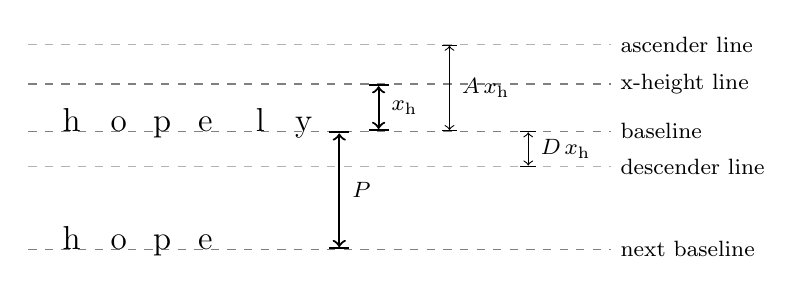
\begin{tikzpicture}[x=1cm,y=1cm,font=\footnotesize]
\draw[dashed,gray]      (0,0)    -- (7.4,0)    node[right,black]{baseline};
\draw[dashed,gray]      (0,0.6)  -- (7.4,0.6)  node[right,black]{x-height line};
\draw[dashed,gray!60]   (0,1.1)  -- (7.4,1.1)  node[right,black]{ascender line};
\draw[dashed,gray!60]   (0,-0.45)-- (7.4,-0.45)node[right,black]{descender line};
\node[anchor=base,font=\large] at (0.55,0) {h};
\node[anchor=base,font=\large] at (1.15,0) {o};
\node[anchor=base,font=\large] at (1.70,0) {p};
\node[anchor=base,font=\large] at (2.25,0) {e};
\node[anchor=base,font=\large] at (2.95,0) {l};
\node[anchor=base,font=\large] at (3.50,0) {y};
\draw[|<->|,thick] (4.45,0) -- (4.45,0.6) node[midway,right=1pt]{$x_{\mathrm{h}}$};
\draw[|<->|] (5.35,0) -- (5.35,1.1)  node[midway,right=1pt]{$A\,x_{\mathrm{h}}$};
\draw[|<->|] (6.35,0) -- (6.35,-0.45)node[midway,right=1pt]{$D\,x_{\mathrm{h}}$};
\draw[dashed,gray] (0,-1.5) -- (7.4,-1.5) node[right,black]{next baseline};
\node[anchor=base,font=\large] at (0.55,-1.5) {h};
\node[anchor=base,font=\large] at (1.15,-1.5) {o};
\node[anchor=base,font=\large] at (1.70,-1.5) {p};
\node[anchor=base,font=\large] at (2.25,-1.5) {e};
\draw[|<->|,thick] (3.95,0) -- (3.95,-1.5) node[midway,right=1pt]{$P$};
\end{tikzpicture}
\caption{The five quantities every subsystem measures handwriting against. $A>1$ because an ascender reaches above the x-height line, and $D<0$ because a descender falls below the baseline. $P$ is the unit used by this block; $x_{\mathrm h}$ is the unit used by every block after it.}
\label{fig:seg-geom}
\end{figure}

\subsubsection{Array primitives: summed-area tables and run tests}

Almost every operation in this block is a sum, a maximum, or a test of whether anything is set, taken over a rectangular window. Computed directly, a window of radius $r$ costs $O(r)$ per pixel per axis, too slow here because the illumination blur below uses a radius of up to 40 pixels. The module therefore builds a summed-area table~\cite{crow1984}, also called an integral image, in one $O(HW)$ pass of two cumulative sums, after which the sum over a window of \emph{any} size costs four look-ups instead of $(2r+1)^2$ additions. Three stages of this block resample an image, and each does so by bilinear interpolation at the source position given by Equation~\ref{eq:seg-resize}, the one exception being an ownership map resampled by nearest neighbour, because its values are integer line indices that interpolation would invent new values for:
\begin{equation}
y_s=\frac{(i+0.5)\,h}{h'}-0.5,\quad x_s=\frac{(j+0.5)\,w}{w'}-0.5,\quad I'(i,j)=\sum_{a,b\in\{0,1\}}\omega_{ab}\,I(\lfloor y_s\rfloor+a,\lfloor x_s\rfloor+b).
\label{eq:seg-resize}
\end{equation}

The table itself is the running two-dimensional sum of the image,
\begin{equation}
S(y,x)=\sum_{i<y}\sum_{j<x} I(i,j),
\label{eq:seg-sat}
\end{equation}
where $S$ is the summed-area table and $I$ the image being summed. Equation~\ref{eq:seg-sat} is built once per image. Any window sum is then read from four of its entries,
\begin{equation}
\mathrm{BoxSum}=S(y_2,x_2)-S(y_1,x_2)-S(y_2,x_1)+S(y_1,x_1),
\label{eq:seg-boxsum}
\end{equation}
where $y_2=y_1+2r+1$ and $x_2=x_1+2r+1$ are the far corners of a window of radius $r$, the array having been padded by $r$ with edge replication beforehand. The cost of Equation~\ref{eq:seg-boxsum} does not depend on $r$, which is what makes the radius-40 illumination blur of Section~3.4.3 affordable.

The same cumulative trick gives the two binary operations the block needs. A dilation along one axis is
\begin{equation}
\mathrm{AnyWithinRadius}(m,r)[i]=\bigl[\,c[i+2r+1]-c[i]>0\,\bigr]=\Bigl[\textstyle\bigvee_{k=-r}^{r} m[i+k]\Bigr],
\label{eq:seg-dilate}
\end{equation}
where $m$ is the binary mask, $c$ its cumulative sum and $r$ the radius. Equation~\ref{eq:seg-dilate} is a dilation because the bracket is true exactly when at least one pixel within $r$ is set. A square dilation separates into two applications of it, one per axis, so it costs the same at any radius. An erosion is the complemented dilation of the complement, and a closing is a dilation followed by an erosion, so no other structuring element has to be implemented. The second operation marks long runs,
\begin{equation}
\mathrm{LongRun}(m,n)[j]=\bigl[\,\mathrm{ch}[h_j+1]-\mathrm{ch}[l_j]>0\,\bigr],\qquad l_j=\max(0,j-n+1),\quad h_j=\min(j,L-n),
\label{eq:seg-runmask}
\end{equation}
where $n$ is the minimum run length, $\mathrm{ch}$ the cumulative count of positions at which a run of $n$ consecutive set pixels begins, $L$ the length of the axis, and $l_j,h_j$ the first and last such start positions that could cover index $j$. Equation~\ref{eq:seg-runmask} is true at every pixel lying on a run of at least $n$ set pixels, and is used by Section~\ref{sec:seg-cleanup} to find printed rules. Figure~\ref{fig:seg-primspseudo} (Appendix~\ref{sec:app-seg}) gives all three as pseudocode. Only one true Gaussian filter is used, a 25-tap kernel smoothing the row profile of Section~\ref{sec:seg-pitchcentres} with $\sigma=4$ rows, about a tenth of a typical pitch.

\subsubsection{Lighting normalisation and binarisation}

The intensity measured by a camera is approximately the reflectance of the paper multiplied by the illumination falling on it. Because the nuisance term is a multiplication and not an addition, it is divided out rather than subtracted: the working grey image $G$ is divided by a single box mean of itself, giving a ratio image $\rho$ close to 1 on paper whatever the lighting, and on ink the ink-to-paper reflectance ratio of the pen itself. Once the shading is divided out, the ink decision is a single global threshold, chosen by Otsu's method~\cite{otsu1979}, which is possible only because of the division --- this is the step that removed the long chain of clean-up filters the project's first segmenter needed.

The ratio image is formed by dividing the grey image by a box mean of itself,
\begin{equation}
\rho(p)=\frac{G(p)}{\max\bigl(\mathrm{BoxMean}_r(G)(p),\,1\bigr)},
\label{eq:seg-flat}
\end{equation}
where $\rho(p)$ is the ratio at pixel $p$, $G$ the working grey image and $\mathrm{BoxMean}_r$ the mean over a window of radius $r$, evaluated through Equation~\ref{eq:seg-boxsum}. The denominator is floored at 1 so a black border cannot divide by zero. The radius is tied to the image height,
\begin{equation}
r=\max\bigl(8,\;\min(40,\;\mathrm{round}(H/41))\bigr),
\label{eq:seg-flatradius}
\end{equation}
where $H$ is the height of the working image in rows. Equation~\ref{eq:seg-flatradius} makes the background estimate cover the same fraction of the page at any camera resolution. The radius must be much larger than a letter, or letters would darken their own background estimate and be divided away; the bounds of 8 and 40 rows keep it so at the resolutions used here.

The threshold separating ink from paper is then the one that best splits the histogram of $\rho$ into two groups, by Otsu's criterion~\cite{otsu1979},
\begin{equation}
t^*=\arg\max_t\;\omega_B(t)\,\omega_F(t)\,\bigl[\mu_B(t)-\mu_F(t)\bigr]^2 ,
\label{eq:seg-otsu}
\end{equation}
where $t^*$ is the chosen threshold, $\omega_B(t)$ and $\omega_F(t)$ are the fractions of pixels below and above a candidate $t$, and $\mu_B(t)$ and $\mu_F(t)$ are their means. The quantity maximised in Equation~\ref{eq:seg-otsu} is the between-class variance, and it is evaluated for all 256 histogram bins at once. A pixel is marked as ink when $\rho<t^*$. Applying Equation~\ref{eq:seg-otsu} globally is defensible only because Equation~\ref{eq:seg-flat} has already removed the shading that would otherwise force a local threshold.

One extra test is needed beyond the threshold: a solid-area veto removes any window entirely ink, since no pen stroke fills a $9\times9$ window, which catches a binder shadow or the dark gutter of a bound book. The whole stage is four array statements (Figure~\ref{fig:seg-inkpseudo}, Appendix~\ref{sec:app-seg}).

\begin{figure}[htb]
\centering
\fbox{\parbox[c][4.5cm]{0.8\linewidth}{\centering [PLACEHOLDER --- four-panel figure: photograph, grey image, blurred background estimate, ratio image $\rho$]}}
\captionsetup{singlelinecheck=false,justification=justified}
\caption{Placeholder: the four stages of Equation~\ref{eq:seg-flat} on one real page --- the photograph, its grey conversion, the box-mean background estimate, and the resulting ratio image $\rho$, showing the shading removed before Otsu's threshold is applied, from \texttt{InkMask}.}
\label{fig:seg-flat-fig}
\end{figure}

\subsubsection{Deskew by searching rotations}

When text lines are horizontal, the row-sum profile of the ink has sharp peaks at the line bodies and deep troughs between them; any tilt smears those peaks, since a single row then cuts across several lines. This projection-profile approach to skew detection~\cite{postl1986} is a standard alternative to a Hough transform over ink edges~\cite{duda1972}, chosen here because a page of handwriting and printed rules gives the Hough transform many competing line candidates, whereas the row profile already favours the direction most of the ink actually runs in. The sharpness of the profile is therefore a measure of how level the page is, and can be maximised directly.

The row profile at a trial angle is the ink count per row,
\begin{equation}
P_\theta(y)=\sum_x R_\theta(y,x),
\label{eq:seg-profile}
\end{equation}
where $P_\theta(y)$ is the number of ink pixels in row $y$ and $R_\theta$ is the ink mask notionally rotated by $\theta$. The sharpness of Equation~\ref{eq:seg-profile} is scored by its sum of squares, and the angle maximising that score is taken,
\begin{equation}
J(\theta)=\sum_y P_\theta(y)^2,\qquad \theta^*=\arg\max_\theta J(\theta),
\label{eq:seg-skew}
\end{equation}
where $J(\theta)$ is the objective and $\theta^*$ the chosen skew angle. Squaring before summing is what makes Equation~\ref{eq:seg-skew} work: the total amount of ink does not change under rotation, so $\sum_yP_\theta(y)$ is fixed, whereas the sum of squares is largest when the same ink is concentrated into the fewest rows, which happens when the lines are level.

The rotation is never performed to score a candidate. Each ink pixel is mapped straight to the row it would land in,
\begin{equation}
k=(y-c_y)\cos\theta-(x-c_x)\sin\theta+c_y,
\label{eq:seg-skewrow}
\end{equation}
where $k$ is that row index, $(y,x)$ the pixel's coordinates and $(c_y,c_x)$ the image centre. Counting rows through Equation~\ref{eq:seg-skewrow} was measured 31 times faster than rotating the mask seventeen times.

The search sweeps 17 candidate angles from $-4^\circ$ to $+4^\circ$ in steps of $0.5^\circ$ on the stage-2 mask reduced by a further factor of two, with no refinement pass, so the best accuracy reachable is half a step, $0.25^\circ$. Ink that would fall outside the row range at a trial angle is allowed to extend the profile rather than being clipped, since clipping piles out-of-range pixels into one row whose artificial spike scores higher than any real text line; an earlier version with this clipping fault chose an angle four degrees wrong on a tilted page. Only once an angle is chosen is the page itself rotated, bilinearly, and the ink mask and ratio image recomputed, because Equation~\ref{eq:seg-flat} is not rotation-equivariant.

Table~\ref{tab:seg-test} (Section~\ref{sec:seg-test}) reports the deskew measurement: seven angles on the search grid recovered exactly in 35 of 35 trials, and four angles between grid points recovered to $0.25^\circ$, exactly half the search step, in 20 of 20 trials, showing the stage is limited by the coarseness of its own search grid and not by the objective.

\subsubsection{Removing what is not handwriting}
\label{sec:seg-cleanup}

Three kinds of nuisance are removed in turn, each identified by a property that handwriting does not share. The area outside the sheet is removed because handwriting disappears under a coarse enough average while the sheet itself does not. Printed structure --- ruled paper, underlines, a bound book's spine shadow --- is removed because it runs straight for longer than a line spacing, which handwriting does not, a long directional opening rather than a fixed-size filter. Edge slivers, corner shadows and creases are removed because, although not straight, they are judged as whole connected pieces rather than pixel by pixel: each fragment is labelled by the same connected-component logic used throughout this block, and the whole piece is then scored on being long and thin or sparse inside its own bounding box.

The long-run primitive of Equation~\ref{eq:seg-runmask}, bracketed by a dilation and a re-intersection with the real ink, gives Equation~\ref{eq:seg-cand} for flat (horizontal) and upright (vertical) printed structure, where $\mathcal D_r^{y}$ and $\mathcal D_r^{x}$ are one-axis dilations:
\begin{equation}
\begin{aligned}
\mathrm{flat}&=\mathcal D_{1}^{y}\Bigl(\mathrm{LongRun}^{x}\bigl(\mathcal D_{1}^{y}(\mathrm{ink}),\;\lfloor1.25P\rfloor\bigr)\Bigr)\wedge\mathrm{ink},\\
\mathrm{upright}&=\mathcal D_{3}^{x}\Bigl(\mathrm{LongRun}^{y}\bigl(\mathcal D_{3}^{x}(\mathrm{ink}),\;\lfloor1.4P\rfloor\bigr)\Bigr)\wedge\mathrm{ink}.
\end{aligned}
\label{eq:seg-cand}
\end{equation}
The two run lengths, $1.25P$ horizontally and $1.4P$ vertically, are longer than any single letter can be, so no letter is mistaken for a rule; the dilation before the run test tolerates a slight tilt, and the re-intersection means only real ink is ever removed.

Separating ink into pieces for the third kind of nuisance needs connected-component labelling: every set pixel is given an integer label, two pixels sharing a label when a path of set pixels joins them. The mask is closed first so pen lifts inside a word are bridged, and the labelling is a run-length union-find pass, each row reduced to its horizontal runs before a union-find structure records which runs belong together, so the whole page is labelled in one pass over the rows. Every discard statistic is accumulated over the \emph{original} ink pixels, not the closed mask, so closing can join pieces but never add area to a decision; eight discard predicates combine size, aspect ratio, faintness and distance from the frame (Table~\ref{tab:seg-artifact}, Appendix~\ref{sec:app-seg}). The most aggressive discards any piece within $\max(3,\lfloor0.5P\rfloor)$ of the left frame edge, which removes the facing page of an open book but costs the first letters of a page with no left margin.

\begin{figure}[htb]
\centering
\fbox{\parbox[c][4cm]{0.75\linewidth}{\centering [PLACEHOLDER --- ruled page before and after rule removal]}}
\captionsetup{singlelinecheck=false,justification=justified}
\caption{Placeholder: a page of ruled paper before and after Equation~\ref{eq:seg-cand} removes the printed rules, confirming that handwriting crossing a rule survives while the rule itself is removed.}
\label{fig:seg-rules}
\end{figure}

\subsubsection{Line pitch and line centres}
\label{sec:seg-pitchcentres}

The row-ink profile is the mask pixel count per row over a central window, smoothed by the Gaussian kernel of Section 3.4.2:
\begin{equation}
\mathrm{prof}(y)=\sum_{x=\lfloor0.05W\rfloor}^{\lfloor0.97W\rfloor-1}\mathrm{ink}(y,x),\qquad \mathrm{sm}=\mathrm{prof}*k,
\label{eq:seg-pitch}
\end{equation}
where $\mathrm{prof}(y)$ is the ink count in row $y$, $W$ is the image width, $k$ is the 25-tap Gaussian kernel of Section~3.4.2 and $\mathrm{sm}$ the smoothed profile. The window in Equation~\ref{eq:seg-pitch} excludes the outer five per cent on the left and three per cent on the right, where a binding shadow or a torn edge would otherwise contribute a constant to every row.

A line centre is a peak of $\mathrm{sm}$ satisfying three conditions together,
\begin{equation}
\mathrm{sm}(y)\ge\mathrm{sm}(y-1),\qquad \mathrm{sm}(y)>\mathrm{sm}(y+1),\qquad \mathrm{sm}(y)>0.06\max_u\mathrm{sm}(u),
\label{eq:seg-centres}
\end{equation}
where $y$ is a candidate row. The comparisons in Equation~\ref{eq:seg-centres} are deliberately asymmetric, one non-strict and one strict, so the last row of a flat-topped peak is taken exactly once. The relative floor of $0.06$ scales with the amount of ink on the page rather than being an absolute count, so a faint page is not rejected wholesale.

The pitch is the median of the gaps between consecutive peaks, used whenever at least two peaks exist; a median rather than a mean so one unusually large gap, such as a paragraph break, cannot shift it. Three fallbacks follow in order when fewer than two peaks are found: the \emph{autocorrelation} of the profile, whose first strong lag in a stated range is taken as the pitch; failing that, an estimate from the median connected-component height, $P=\max(15,\mathrm{round}(2.2\,\mathrm{median}\{h_c\}))$; and, with no usable components either, a fixed 48 rows (Figure~\ref{fig:seg-pitchpseudo}, Appendix~\ref{sec:app-seg}). The pitch and profile are recomputed on the cleaned mask after Section~\ref{sec:seg-cleanup}, and the peaks become line centres through greedy non-maximum suppression, a peak accepted only if it lies at least $0.6P$ from every centre already accepted.

Table~\ref{tab:seg-test} reports the line-count test below.

\subsubsection{Seam cut, pixel ownership and the final crop}

A straight cut halfway between two line centres would sever every descender and ascender that crosses it, so the boundary between two lines must bend around the ink. The two layers of ink recovery --- a strict page-wide mask and a looser threshold trusted only next to ink a line already owns --- exist because a threshold loose enough to catch a faint stroke is also loose enough to catch a shadow, and \emph{hysteresis}, using two thresholds instead of one, is the standard remedy, the same principle used to link edges in edge detection applied here to ink.

The boundary itself is found the way a seam is found in content-aware image resizing: the cheapest vertical path across a cost image, found column by column with dynamic programming rather than guessed as a straight line~\cite{avidan2007}. Between consecutive centres $c_0<c_1$ the cost field of Equation~\ref{eq:seg-cost2} and the dynamic-programme recursion of Equation~\ref{eq:seg-seam} give the cheapest path across it:
\begin{equation}
C(y,x)=4.0\,\tilde m(y,x)+0.012\left(\frac{y-\mu}{\max(1,(c_1-c_0)/2)}\right)^{\!2},\qquad \mu=c_0+\tfrac12(c_1-c_0),
\label{eq:seg-cost2}
\end{equation}
where $C(y,x)$ is the cost of placing the boundary at row $y$ of column $x$, $\tilde m$ is the dilated ink mask, and $\mu$ is the midline between the two centres $c_0$ and $c_1$. The two weights in Equation~\ref{eq:seg-cost2} are three hundred to one: crossing a single ink pixel costs 4.0 against a maximum of 0.012 for sitting a half-gap away from the midline, so the midline term only breaks ties across blank gaps between words and never persuades the seam to cut a letter.

The cheapest path is accumulated column by column,
\begin{equation}
A(y,x)=C(y,x)+\min_{|d|\le s}\bigl[\,A(y+d,\,x-1)+0.02\,|d|\,\bigr],\qquad A(y,0)=C(y,0),
\label{eq:seg-seam}
\end{equation}
where $A(y,x)$ is the cost of the cheapest path reaching $(y,x)$, $d$ is the row step taken between adjacent columns and $s=7$ bounds it. The penalty $0.02\,|d|$ in Equation~\ref{eq:seg-seam} prices vertical movement, so the seam prefers to stay level unless ink gives it a reason to climb.

The crop is then composited from its layers by a hysteresis rule,
\begin{equation}
\alpha=\max\Bigl(\alpha_{\mathrm{strong}},\ \ \mathbb 1[\rho_{\mathrm{local}}<t^*_{\mathrm{local}}]\cdot\alpha_{\mathrm{halo}}\cdot\mathbb 1[\text{not owned by another band}]\Bigr),
\label{eq:seg-hyst}
\end{equation}
where $\alpha$ is the opacity written into the crop, $\alpha_{\mathrm{strong}}$ comes from the page-wide mask, $\alpha_{\mathrm{halo}}$ from the looser local threshold $t^*_{\mathrm{local}}$, and $\mathbb 1[\cdot]$ is 1 when its condition holds and 0 otherwise. The second term of Equation~\ref{eq:seg-hyst} is the loose layer, admitted only next to ink the band already owns, which is the hysteresis: a faint stroke touching known ink is kept, while an equally faint shadow elsewhere is not.

Finally the crop's contrast is stretched,
\begin{equation}
\ell=\mathrm{clip}\!\left(\frac{255\,(v-b)}{\max(w-b,1)},0,255\right),\qquad
\mathrm{out}=255\Bigl(1-\bigl(\tfrac{255-\ell}{255}\bigr)^{0.55}\Bigr),
\label{eq:seg-stretch}
\end{equation}
where $v$ is the input grey value, $b$ and $w$ are the black and white points taken from the crop's own histogram, $\ell$ is the linearly stretched value and $\mathrm{out}$ the value written. The exponent $0.55$ in Equation~\ref{eq:seg-stretch} thickens thin strokes slightly, which matters because the recogniser was trained on ink of a similar weight.

The two outermost boundaries are fixed at $\lfloor0.75P\rfloor$ beyond the first and last centre, so $L$ centres give exactly $L$ bands; the whole computation is $O(15HW)$ at worst, the most expensive single step in the block. A pixel belongs by default to the band it lies in; six correction rules on top return a cut-off tail to the band holding most of its piece, place a small fragment by proximity, and follow a dot or accent down to its stem (Table~\ref{tab:seg-own}, Appendix~\ref{sec:app-seg}). Each crop is rendered from the full-resolution page and composited from three layers: the band's own ink mask, a recovery mask from re-applying Equations~\ref{eq:seg-flat} and~\ref{eq:seg-otsu} inside the crop alone, and the halo of the band's own strong ink. Outside the mask the crop is pure white, and it is shifted so the first inked column sits at a fixed offset, since the recogniser's input is left-flush (Equation~\ref{eq:seg-clf}):
\begin{equation}
s=\min\!\Bigl(\frac{64}{h},\frac{640}{w}\Bigr),\qquad h'=\max(1,\mathrm{round}(hs)),\qquad w'=\max(1,\mathrm{round}(ws)).\label{eq:seg-clf}
\end{equation}

\subsubsection{Testing the segmentation block}
\label{sec:seg-test}

Two properties of this block were tested against a known answer on the 30 photographed pages of the five personal writers, $2448\times3264$ pixels each. Table~\ref{tab:seg-test} gives the results: the block found the correct number of lines on all 30 pages, 669 of 669 lines, with no page over- or under-segmented, against the hand-typed transcription; and the deskew of Equation~\ref{eq:seg-skew} recovered seven grid-aligned injected angles exactly in 35 of 35 trials and four off-grid angles to $0.25^\circ$ in 20 of 20 trials.

\begin{table}[h]
\centering
\fontsize{9}{11}\selectfont
\setlength{\tabcolsep}{4pt}
\begin{tabularx}{\linewidth}{|p{4.3cm}|p{3.3cm}|X|}
\hline
\textbf{Measurement} & \textbf{Result} & \textbf{What it shows} \\
\hline
Line count against the hand-typed transcription, 30 pages & \textbf{30 of 30} pages exact; 669 of 669 lines & The line separation is correct on every page tested, and the relative floor of Equation~\ref{eq:seg-centres} lost no line. \\
\hline
Deskew, 7 angles on the search grid, 5 pages & \textbf{35 of 35} exact & The objective of Equation~\ref{eq:seg-skew} picks the correct grid point every time. \\
\hline
Deskew, 4 angles between grid points, 5 pages & \textbf{20 of 20} at $0.25^\circ$ & The residual error is exactly half the search step, so the stage is quantisation-limited, not objective-limited. \\
\hline
Time per page, $2448\times3264$ & \textbf{4.9 to 9.7\,s}, mean 7.9\,s & The cost of the deployed module. Measured with the project's own resampling throughout. \\
\hline
Measured line pitch $P$ & 47 to 58 pixels & The scale unit varies by 23\,\% across these writers, which is what the block is designed to absorb. \\
\hline
Chosen skew angle on the unrotated pages & $-1.5^\circ$ to $+3.0^\circ$ & Real photographs are tilted by more than a degree, so the stage is doing necessary work. \\
\hline
\end{tabularx}
\caption{Measured performance of the deployed segmentation block over the 30 photographed pages of the five personal writers. These are the pages the system was built on, not an unseen test set, so the line-count result shows that the block handles the material it was designed for and not that it generalises to new conditions.}
\label{tab:seg-test}
\end{table}

The 30 pages are the pages the system was built on, so the line-count result is not an unseen test; the deskew result is stronger, since the injected angle is ground truth no part of the design could have been fitted to. The timing figure also corrects an attribution: the 24.8 to 69.1\,s per page reported in Section~\ref{sec:results} is the retired segmenter, \texttt{SegmentPage.ProcessPage}; the deployed module is roughly five times faster at 4.9 to 9.7\,s, because it makes one pass over a half-resolution image where the retired module made four passes over a larger one. The mean of 7.9\,s is still about four times the two seconds requirement R4 allows for capture and conditioning. Using the project's own resampling rather than the imaging library's compiled resampling costs about 40\,\% of the block's run time, the measured price of the library-free claim.
\mustdo{update the segmentation figures of Section~\ref{sec:results} and the R4 budget to 4.9--9.7\,s; time \texttt{SegmentLean.SegmentLines} on the ODROID N2+; produce the four figures placeholdered above, plus the paper-region mask and the \texttt{\_cuts\_overlay.jpg} that \texttt{SegmentLean.py} already writes.}

\begin{figure}[htb]
\centering
\fbox{\parbox[c][5cm]{0.85\linewidth}{\centering [PLACEHOLDER --- one full page with the final seam cuts overlaid in colour, from \texttt{SegmentLean.py}'s own debug output]}}
\captionsetup{singlelinecheck=false,justification=justified}
\caption{Placeholder: the seam-cut overlay (\texttt{\_cuts\_overlay.jpg}) on one real, photographed page, showing each line's final boundary bending around ascenders and descenders rather than cutting straight through them.}
\label{fig:seg-cuts}
\end{figure}

\subsubsection{Design alternatives and limitations}

Table~\ref{tab:seg-alt} sets the main design choices against the alternatives considered. The project's first segmenter, \texttt{SegmentPage.py}, was about 2200 lines and sixty functions against the eleven here; it resized every photograph to a fixed long side, thresholded locally, removed printed structure in four passes, took a median glyph height as its scale unit, scored components for being diagrams, chained them into lines and deskewed each line separately. No part of the deployed pipeline calls it any more, and three of its capabilities were given up with it: diagram tagging, per-line deskew, and a wider $\pm8^\circ$ search at $0.1^\circ$.

\begin{table}[h]
\centering
\fontsize{8.5}{10.2}\selectfont
\setlength{\tabcolsep}{4pt}
\begin{tabularx}{\linewidth}{|p{2.4cm}|X|}
\hline
\textbf{Decision} & \textbf{Alternatives, and why the deployed choice was made} \\
\hline
Lighting & Subtracting a blurred background leaves contrast dependent on brightness. The nuisance is multiplicative, so dividing gives an ink-to-paper ratio independent of the lamp. \\
\hline
Ink threshold & A local mean less an offset marks something even in an empty region and needs a tuned offset. After the division, one global Otsu threshold is enough. \\
\hline
Scale unit & A median glyph height is upset by a heading in another size; a fixed-size page throws away resolution. The pitch $P$ is measured on the page itself. \\
\hline
Lines & Chaining components along a baseline curve needs a correct set of components first, propagating every clean-up error. The row profile yields the pitch and centres together in one $O(N_p)$ pass. \\
\hline
Line boundaries & A straight cut at the midline severs descenders and ascenders. The least-ink seam bends around them. \\
\hline
Skew & A Hough transform of ink edges~\cite{duda1972} is dominated by ruled lines and diagram strokes. The projection objective is also the quantity the pitch stage goes on to use, so it costs nothing extra. \\
\hline
Rule removal & A long morphological opening erases underlines and cannot follow a slope. The dilated long-run test needs two constants where chaining fragments across gaps needs five. \\
\hline
Not implemented & Text-versus-diagram tagging, per-line deskew and a four-point perspective warp are all absent; the first is accepted for plain prose pages, the residual drift is tolerated downstream, and the camera looks straight down. \\
\hline
\end{tabularx}
\caption{Design alternatives of the deployed segmentation block. The last row records capabilities of the first segmenter that were deliberately given up.}
\label{tab:seg-alt}
\end{table}

The block assumes left-to-right writing in a single column of roughly horizontal lines, and the following limitations follow from that design. Skew beyond $\pm4^\circ$ is not corrected at all, and up to $0.25^\circ$ always remains. Two columns of text, or a diagram beside the text, produce profile peaks that belong to no single line, and an untagged diagram is cut into line-shaped crops and read as nonsense. A line peaking below six per cent of the strongest is lost silently, although no such line occurred in the 30 pages tested. A blank page raises an exception rather than returning no lines. Illumination varying faster than the radius of Equation~\ref{eq:seg-flat} leaves one side of a hard shadow edge mis-thresholded, page curl and perspective are untreated, and colour is treated like black ink because the module is monochrome throughout.


\subsection{Text recognition and writer identification}
\label{sec:textrec}
\label{sec:writerid}

This subsection describes the two neural networks that read a handwritten line into text and decide which of the thirteen stored writers wrote it (functional unit FU~2.3; requirements R1, R2), component by component: the convolutional backbone the two share, the sequence model and alignment-free loss that make text recognition possible at all, the writer-identification head and the stroke normalisation it depends on, and the from-scratch training and verification of every layer. No machine-learning library is used anywhere in this subsection: the forward passes, the backward passes and the optimiser updates are all evaluated by one module written for this project, \texttt{NumpyNN.py} (Section~\ref{sec:textrec-numpynn}).

Both networks follow the layer pattern of Kizilirmak and Yanikoglu~\cite{kizilirmak2023}, chosen because it was evaluated on the public handwriting database used here~\cite{marti2002} and reports accuracies in the range R2 needs. That paper describes an approach and a layer pattern rather than publishing code, so the network was built from its description: the layer pattern, filter counts and recurrent width are taken from it, while the input geometry, data pipeline, label cleaning, augmentation and staged training recipe were decided for this project. That hybrid of convolution and recurrence is the combination reported to improve feature extraction and contextual understanding together~\cite{kumar2024,ma2023}.

\subsubsection{The shared convolutional backbone}
\label{sec:rec-backbone}

A convolutional neural network (CNN) is a stack of layers each of which applies the same small learned filter at every position of its input~\cite{lecun1998,yahya2021}. Applying one filter everywhere, rather than learning a separate weight for every pixel, is what makes the layer useful for handwriting: a stroke junction means the same thing wherever on the line it appears, so the filter that detects it should not have to be learned again for each position. A single convolutional layer only sees a small local neighbourhood, but stacking several lets later layers combine the simple strokes earlier layers detect into the more complex shapes of whole letters, which is why depth rather than one wide layer is used. Three further layer types complete the pattern used here, each solving a specific problem of training a deep stack: \emph{batch normalisation}, the \emph{rectifier} nonlinearity, and \emph{pooling}.

A convolution with kernel size $k$, stride $s$ and $p$ rows and columns of zero padding on each side of input $X_{\mathrm{pad}}$ is
\begin{align}
Y[o,i,j]&=b_o+\sum_{c=1}^{C_{\mathrm{in}}}\sum_{u=0}^{k-1}\sum_{v=0}^{k-1}W[o,c,u,v]\;X_{\mathrm{pad}}[c,\,s\,i+u,\,s\,j+v],\label{eq:rec-conv}\\
Y&=\tilde W\,\mathrm{cols}+b\,\mathbf 1^{\top}.\label{eq:rec-im2col}
\end{align}
Equation~\ref{eq:rec-conv} is six nested summations, too slow in array arithmetic, so the implementation uses the \emph{im2col} rearrangement of Equation~\ref{eq:rec-im2col}: every $k\times k$ patch the filter would see is copied out as one column, the filter weights reshaped into rows, and the whole convolution becomes a single matrix product, agreeing with the direct form to about $10^{-13}$ and about ten times faster. With $k=3$, $p=1$, $s=1$ the output keeps the input's height and width, so only pooling layers change the tensor size. Batch normalisation~\cite{ioffe2015} (Equation~\ref{eq:rec-bn}) rescales each channel to zero mean and unit variance over the current training batch and then applies a learned scale $\gamma$ and shift $\beta$; at inference, with no batch to average over, running statistics collected during training replace $\mu_B,\sigma_B^2$ and the whole operation folds into the single affine map of Equation~\ref{eq:rec-bnfold}:
\begin{align}
\hat x&=\frac{x-\mu_B}{\sqrt{\sigma_B^2+\varepsilon}},\qquad y=\gamma\hat x+\beta,\qquad\varepsilon=10^{-5},\label{eq:rec-bn}\\
a&=\frac{\gamma}{\sqrt{\sigma^2_{\mathrm{run}}+\varepsilon}},\qquad b=\beta-a\,\mu_{\mathrm{run}},\qquad y=a\,x+b.\label{eq:rec-bnfold}
\end{align}
The rectifier is $\max(0,x)$~\cite{nair2010}: some nonlinearity is essential, because a stack of purely linear layers collapses into one linear layer however deep it is, and the rectifier's derivative of 0 or 1 neither saturates nor shrinks the gradient across twelve layers. Max-pooling takes the largest value in each $2\times2$ window, stride 2, halving both axes with no learned parameters~\cite{ji2021}; it discards three quarters of the positions, keeping the network small enough for the target hardware, and tolerates a one-pixel shift, since moving a stroke slightly usually does not change which value in its window is largest.

Figure~\ref{fig:rec-arch} gives the three convolutional stages (32, 64 and 128 channels, 2, 4 and 6 layers respectively) with two intervening max-pools, each verified for this project against the published pattern; what follows the backbone differs between the two networks and is given in Sections~\ref{sec:rec-ctc} and~\ref{sec:wid-head}. The full recogniser holds 3\,358\,763 trainable parameters, of which the recurrent layers hold 70.5\,\% and the third convolutional stage 24.2\,\% (Table~\ref{tab:rec-layers}, Appendix~\ref{sec:app-rec}); these shapes cost $4.17\times10^9$ multiply--accumulates per line, $3.79\times10^9$ of them convolutional, so the convolutions dominate the arithmetic even though the recurrent layers hold most of the parameters.

\begin{figure}[h]
\centering
\begin{tikzpicture}[x=1cm,y=1cm,scale=0.86,transform shape]
\tikzset{nb/.style={w2box,text width=2.55cm,minimum height=1.5cm}}
\node[nb] (in) at (-6.2,0) {\textbf{Input}\\ $1\times64\times640$};
\node[nb] (s1) at (-3.1,0) {\textbf{Stage 1}\\ 2$\times$[conv 3$\times$3, BN, ReLU], 32 ch.\\ $32\times64\times640$};
\node[nb] (p1) at (0,0) {\textbf{Max-pool 2$\times$2}\\ $32\times32\times320$};
\node[nb] (s2) at (3.1,0) {\textbf{Stage 2}\\ 4$\times$[conv, BN, ReLU], 64 ch.\\ $64\times32\times320$};
\node[nb] (p2) at (6.2,0) {\textbf{Max-pool 2$\times$2}\\ $64\times16\times160$};
\node[nb] (s3) at (6.2,-2.3) {\textbf{Stage 3}\\ 6$\times$[conv, BN, ReLU], 128 ch.\\ $128\times16\times160$};
\node[nb] (hm) at (3.1,-2.3) {\textbf{Height max-pool}\\ $128\times1\times160$\\ $\rightarrow$ 160 vectors};
\node[nb] (ls) at (0,-2.3) {\textbf{text: BiLSTM $\times2$}\\ \textbf{writer: pool + head}\\ (Sections~\ref{sec:rec-ctc}, \ref{sec:wid-head})};
\foreach \a/\b in {in/s1,s1/p1,p1/s2,s2/p2,p2/s3,s3/hm,hm/ls} \draw[w2arr] (\a)--(\b);
\end{tikzpicture}
\caption{The shared convolutional backbone, the layer pattern being that of Kizilirmak and Yanikoglu~\cite{kizilirmak2023}. Tensor shapes are channels $\times$ height $\times$ width; BN denotes batch normalisation. The two height-collapsed feature sequences feed the text recogniser's recurrent stage and the writer classifier's pooling head respectively.}
\label{fig:rec-arch}
\end{figure}

Both networks share one input convention rather than each defining its own. Every crop, for either network, is resized uniformly to fit a $64\times640$ canvas, pasted left-aligned and vertically centred, inverted and normalised so paper is $-1$ and ink $+1$ (Equations~\ref{eq:rec-resize}, \ref{eq:rec-norm}):
\begin{align}
s&=\min\!\Bigl(\frac{64}{h},\frac{640}{w}\Bigr),\qquad w'=\max(1,\mathrm{round}(ws)),\qquad h'=\max(1,\mathrm{round}(hs)),\label{eq:rec-resize}\\
x&=\frac{(1-p/255)-0.5}{0.5}=1-\frac{2p}{255}.\label{eq:rec-norm}
\end{align}
A single scale factor on both axes avoids distorting letter proportions, a plain stretch having first been tried and rejected for exactly that reason; the left flush makes the map from a network column back to a crop pixel the exact inverse $x_{\mathrm{orig}}=x_{\mathrm{canvas}}/s$, which Section~\ref{sec:styleprofile} depends on.

Before the eval-mode form was trusted on the single-board computer it was cross-checked against the training-mode forward pass on the same weights with statistics frozen: over 1358 real lines the top-1 agreement was 100.00\,\% with a maximum absolute logit difference of $7.6\times10^{-6}$, confirming Equation~\ref{eq:rec-bnfold}'s folded form reproduces Equation~\ref{eq:rec-bn} to within numerical noise.

\subsubsection{Sequence modelling and text recognition by CTC}
\label{sec:rec-ctc}

The input is one grey-scale line image; the output is the string that was written. Three properties of handwriting fix the design: cursive characters are joined, so their boundaries cannot be located reliably and cutting the line into characters, as the proposal planned, would pass every cutting error into a wrong reading; the number of characters is unknown and has no fixed relation to image width; and the available training material gives line images with transcriptions, but not the position of every character. The convolutional backbone gives one feature vector per narrow vertical slice of the line, via the height max-pool $z_t[c]=\max_iF[c,i,t]$, $t=1,\ldots,T=160$, a maximum because the question is only whether a feature occurs anywhere in that column, which should answer the same way for an ascender and a short letter. A plain recurrent network multiplies by the same weight matrix every step, so a gradient over a long sequence either shrinks away or grows without bound; a long short-term memory cell~\cite{hochreiter1997} avoids this by carrying a cell state forward by addition, $c_t=f_t\odot c_{t-1}+i_t\odot g_t$, through three learned gates, so a gradient can cross many steps without vanishing. A \emph{bidirectional} layer~\cite{schuster1997} runs a second pass over the reversed sequence and concatenates both outputs, necessary for joined handwriting where strokes such as those of u, n and m are nearly identical locally and can only be told apart from what follows.

This bidirectional-recurrent, alignment-free combination is the one that established accurate unconstrained handwriting recognition from whole lines rather than cut characters~\cite{graves2009}. Connectionist temporal classification~\cite{graves2006} is what makes training possible from line transcriptions alone, with no character-level labels: rather than scoring the single alignment that happens to be correct, it sums the probability of \emph{every} alignment (\emph{path}) that would produce the right transcription, using a 75th \emph{blank} symbol so that a genuine doubled letter is not merged away by the path-collapse rule.

The recurrent output at each step is turned into a distribution over the symbol set by a linear layer and a log-softmax,
\begin{equation}
\ell_t=W_oh_t+b_o,\qquad \log y_t^k=\ell_t^k-\log\sum_{j=0}^{74}e^{\ell_t^j},
\label{eq:rec-softmax}
\end{equation}
where $h_t$ is the recurrent output at step $t$, $W_o$ and $b_o$ the output weights and bias, $\ell_t$ the logits, and $y_t^k$ the probability of symbol $k$ at step $t$. Equation~\ref{eq:rec-softmax} is evaluated in log form, subtracting the log-sum-exp rather than dividing by the sum, because the probabilities are multiplied over 160 steps and would underflow in a linear representation.

The probability of a transcription is then the summed probability of every path that collapses onto it,
\begin{equation}
P(\pi\mid x)=\prod_{t=1}^{T}y_t^{\pi_t},\qquad p(y\mid x)=\!\!\sum_{\pi:\,\mathcal B(\pi)=y}\!\!P(\pi\mid x),\qquad \mathcal L_{\mathrm{CTC}}=-\ln p(y\mid x),
\label{eq:rec-ctcprob}
\end{equation}
where $\pi$ is one path through the lattice, $x$ the input line, $y$ the transcription, $\mathcal B$ the collapse map that merges repeats and deletes blanks so that $\mathcal B(\text{--hh-e-ll-ll-o})=\text{hello}$, and $\mathcal L_{\mathrm{CTC}}$ the training loss. The number of paths grows exponentially with $T$, so the sum in Equation~\ref{eq:rec-ctcprob} is evaluated by a forward--backward dynamic programme~\cite{graves2006} costing $O(TU)$ for a transcription of $U$ characters, which also yields the training gradient in closed form as the difference between what the network predicted and what the alignment lattice expects.

At inference the alignment no longer matters and the most probable symbol per step is taken directly,
\begin{equation}
\hat\pi_t=\arg\max_k y_t^k,\qquad \hat y=\mathcal B(\hat\pi),
\label{eq:rec-greedy}
\end{equation}
where $\hat\pi$ is the best path and $\hat y$ the string read back. Equation~\ref{eq:rec-greedy} is best-path, or \emph{greedy}, decoding, used here with no lexicon, language model or beam search, so nothing in the system corrects a misspelling; every error reported in Section~\ref{sec:results} is the network's own.

The 74 symbols are the 26 lower- and upper-case letters, the ten digits and twelve punctuation symbols; class 0 is the blank. Training minimises the CTC loss by mini-batch RMSprop~\cite{tieleman2012} with weight decay, gradient-norm clipping at 5 against the exploding gradients a long recurrent unroll can produce~\cite{pascanu2013}, and a plateau learning-rate schedule, in the four stages of Table~\ref{tab:rec-stages}, each motivated by a limitation of the previous one: the base stage reproduced the published recipe on lines cut by this project's own tools; the clean-label stage warm-started from it on the public set; fine-tuning on the personal lines alone was rejected because it cut general accuracy by about ten points, catastrophic forgetting barely reduced by freezing the convolutions; and the joint stage therefore continues on both sets at once with a weighted sampler giving each personal line weight $f/n_P$ and each public line $(1-f)/n_T$, $f=0.20$.

\begin{table}[h]
\centering
\fontsize{8.5}{10.2}\selectfont
\setlength{\tabcolsep}{4pt}
\begin{tabularx}{\linewidth}{|p{1.8cm}|p{1.4cm}|X|p{3.4cm}|}
\hline
\textbf{Stage} & \textbf{Data} & \textbf{Schedule and selection} & \textbf{Checkpoint and character accuracy} \\
\hline
1 Base & own lines & $\eta_0=10^{-3}$, batch 16, halve after 5 stalls; best validation loss & best validation loss 1.06 per line \\
\hline
2 Clean labels & public set & as above, up to 8 restarts; best public validation loss & \texttt{hf\_best}: 93.87 / 91.60\,\% public validation / test \\
\hline
3 Personal (rejected) & personal lines & $\eta_0=3\times10^{-4}$, 60 epochs; best personal validation loss & \texttt{personal\_best}: 84.26\,\% public, 90.2\,\% personal \\
\hline
4 Joint & both, $f=0.20$ & $\eta_0=5\times10^{-4}$, 30 epochs, clip 5; best $\min$ of both accuracies & \texttt{joint\_best}: 94.03 / 91.82\,\% public, 89.64\,\% personal \\
\hline
\end{tabularx}
\caption{The four training stages, with the character accuracies measured on each stage's own checkpoint. All stages use RMSprop with weight decay $10^{-5}$. None of these figures was measured on \texttt{paper\_cnn\_bilstm\_ctc\_scratch\_best.npz}, the file the deployed loader actually prefers (Section~\ref{sec:rec-ctc-limits}).}
\label{tab:rec-stages}
\end{table}

\emph{Augmentation}, distorting each training image slightly and differently every time it is used so the network cannot memorise it, applies at most one of shear, rotation, elastic distortion or perspective distortion per training image, never to validation or test images.

Table~\ref{tab:rec-results} gives the measured accuracy. On the public test partition (2\,915 lines, used for no decision) the recogniser reaches 91.82\,\% character accuracy; on 669 correctly cut personal crops, 98.61\,\% character and 94.21\,\% word accuracy; through the complete page-to-text pipeline including segmentation, 61.21\,\%, the largest discrepancy in this report and only partly attributable to recognition itself, since the two figures used different recogniser versions (Section~\ref{sec:rec-ctc-limits}). Recognition speed measured 8.86\,ms per character over 669 real crops, inside the 25\,ms per character of R4 by about 2.8 times on the development laptop; timing on the ODROID N2+ was not measured. \mustdo{measure recognition time per line on the ODROID N2+.}

\begin{table}[h]
\centering
\fontsize{8.5}{10.2}\selectfont
\setlength{\tabcolsep}{4pt}
\begin{tabularx}{\linewidth}{|p{3.1cm}|p{2.7cm}|X|}
\hline
\textbf{Data set} & \textbf{Result} & \textbf{Status of the figure} \\
\hline
Public set, test (2\,915 lines) & 91.82\,\% character; WER 26.7\,\% & Used for no decision; the cleanest general-benchmark figure. \\
\hline
Personal crops, 669 correctly cut lines & 98.61\,\% character, 94.21\,\% word & Writers appear in fine-tuning data; the operating figure of Section~\ref{sec:results}. \\
\hline
Full page pipeline, ten personal pages & 61.21\,\% (CER 38.79\,\%) & Only figure exercising the complete page-to-text chain; earlier recogniser version. \\
\hline
Recognition speed, 669 crops & 8.86\,ms/character, 353\,ms/line & Margin of about 2.8$\times$ against R4 on the laptop; not measured on the board. \\
\hline
\end{tabularx}
\caption{Accuracy and speed of the text recogniser. See Table~\ref{tab:rec-results} of Appendix~\ref{sec:app-rec} for the full per-writer breakdown.}
\label{tab:rec-results}
\end{table}

\label{sec:rec-ctc-limits}
The recognition head carries two limitations that bear directly on how its figures should be read. Four text checkpoints exist; the deployed loader prefers \texttt{paper\_cnn\_bilstm\_ctc\_scratch\_best.npz}, the output of the from-scratch trainer of Section~\ref{sec:textrec-numpynn}, whose accuracy was never logged, so no figure in this report is measured on the exact file the deployed system uses --- the figures above describe the joint checkpoint. \mustdo{evaluate the scratch checkpoint and quote its figures beside the joint ones, or name the single checkpoint being submitted.} Correcting the evaluation labels alone raised an early ten-author hold-out accuracy from 42.7\,\% to 89.4\,\%, showing label quality rather than the network limited the earliest measurements. The CTC routine does not survive an empty label sequence, a confined indexing fault rather than an algorithmic one.

\subsubsection{Writer-identification head and stroke normalisation}
\label{sec:wid-head}
\label{sec:wid-strokenorm}

The task is closed-set: choose one of $K=13$ known writers from a line image. A classifier trained on raw grey-scale crops read real held-out lines at 99.78\,\% over 1358 lines but identified the writer of \emph{synthesised} output in only about 28\,\% of trials, because the plotter draws every stroke at one width and one pressure while real handwriting carries a thickness and ink density a convolutional network readily exploits when training lines are few, and such a judge predicts neither what the machine can draw nor how a reader recognises a hand, which is by geometry. A second classifier was therefore trained on \emph{stroke-normalised} crops, in which thickness is removed by construction: the ink classifier serves real photographed pages, the shape classifier the best-of-$N$ search of Section~\ref{sec:synthesis}.

The writer-identification head differs from the recogniser's in one deliberate way: the recurrent layers are not used, because a writer's slant and stroke habits do not depend on the order the letters come in, so adding sequence information would only cost parameters.

The head pools the backbone's feature map twice, deliberately with two different operations,
\begin{equation}
m_{c,t}=\max_{r=1,\ldots,16}F_{c,r,t},\qquad f_c=\frac1{160}\sum_{t=1}^{160}m_{c,t},\qquad f\in\mathbb R^{128},
\label{eq:wid-pool}
\end{equation}
where $F_{c,r,t}$ is the backbone feature map at channel $c$, row $r$ and column $t$, $m_{c,t}$ the height-pooled map and $f_c$ the final descriptor for channel $c$. The two operations in Equation~\ref{eq:wid-pool} answer two different questions. The height \emph{maximum} asks whether a stroke pattern occurs anywhere in a column, as in the recogniser. The width \emph{mean} asks how \emph{often} it occurs along the whole line, which is the right question for a habit rather than a one-off accident; a maximum there would answer only whether the writer ever made the stroke once.

The descriptor is then mapped to one score per writer by two linear layers,
\begin{equation}
h=\mathrm{ReLU}(W_1f+b_1)\in\mathbb R^{96},\qquad z=W_2\,\mathrm{Drop}_{0.2}(h)+b_2\in\mathbb R^{K},
\label{eq:wid-head}
\end{equation}
where $W_1,b_1,W_2,b_2$ are the learned weights and biases, $h$ the hidden activation, $\mathrm{Drop}_{0.2}$ dropout at rate $0.2$ and $z$ the $K$ logits. The dropout in Equation~\ref{eq:wid-head}~\cite{srivastava2014} is active only during training, and stops the small head memorising individual lines when only 63 to 184 lines exist per writer. Training uses the cross-entropy loss, Equation~\ref{eq:wid-ce}, whose gradient with respect to the logits is the simple form of Equation~\ref{eq:wid-cebw}:
\begin{align}
p_k&=\frac{e^{z_k}}{\sum_{j=1}^{K}e^{z_j}},\qquad
\mathcal L=\frac1B\sum_{n=1}^B\Bigl[\log\sum_je^{z^{(n)}_j}-z^{(n)}_{y_n}\Bigr],\qquad\hat k=\arg\max_kp_k,\label{eq:wid-ce}\\
\frac{\partial\mathcal L}{\partial z^{(n)}_k}&=\frac{1}{B}\bigl(p^{(n)}_k-\mathbb 1[k=y_n]\bigr).\label{eq:wid-cebw}
\end{align}
\emph{Stroke normalisation} re-draws a line at a constant pen width proportional to its own letter height, by Otsu binarisation~\cite{otsu1979}, rule removal, the core-band x-height estimate of Equation~\ref{eq:wid-xh}, closing of hairline breaks, Zhang--Suen thinning~\cite{zhang1984}, and re-inking at a width $w=\mathrm{clip}(\mathrm{round}(0.14\,x_h),2,9)$ independent of scan resolution:
\begin{equation}
H_{\mathrm{run}}\ge\max(24,\lfloor1.1h\rfloor)\ \wedge\ V_{\mathrm{run}}\le\max(3,\lfloor0.12h\rfloor),\qquad
x_h=\text{base}-\text{top}.
\label{eq:wid-xh}
\end{equation}

The two classifiers hold 966\,445 parameters each, the ink classifier trained end to end from the recogniser backbone, the shape classifier also trained end to end after an earlier frozen-backbone configuration proved a training fault (Section~\ref{sec:later-endtoend}). On a real photograph the ink classifier's line probabilities are averaged across the page, Equation~\ref{eq:wid-aggr}, with no weighting by length or confidence:
\begin{equation}
\bar p_k=\frac1N\sum_{n=1}^Np^{(n)}_k,\qquad\hat k=\arg\max_k\bar p_k,\qquad\text{confidence}=100\,\bar p_{\hat k}\ \%.
\label{eq:wid-aggr}
\end{equation}
For synthesised output the shape classifier's probability for the target writer becomes one term of the best-of-$N$ score of Section~\ref{sec:syn-search} instead.

\begin{figure}[htb]
\centering
\fbox{\parbox[c][4.5cm]{0.85\linewidth}{\centering [PLACEHOLDER --- one real cursive line and one disconnected line, each shown as grey crop, Otsu mask with rules removed, core band with $x_h$ marked, skeleton, and final re-inked constant-width canvas]}}
\captionsetup{singlelinecheck=false,justification=justified}
\caption{Placeholder: the six steps of stroke normalisation (\texttt{StrokeNormalize}) applied to one database line and one personal line, showing slant, proportions and connection habits surviving while pen thickness is removed, for a disconnected and a strongly cursive hand side by side.}
\label{fig:wid-snorm-fig}
\end{figure}

Table~\ref{tab:wid-results} gives the measurements that motivated the design; chance level for thirteen writers is 7.7\,\%. The ink classifier reaches 99.78\,\% over 1358 real lines; the shape classifier, after the end-to-end correction of Section~\ref{sec:later-endtoend}, 93.67\,\% on the same lines, up from 83.36\,\% under the superseded frozen-backbone recipe, where 118 of one writer's 148 lines had gone to a single neighbour.

\begin{table}[!htbp]
\centering
\fontsize{8}{9.6}\selectfont
\setlength{\tabcolsep}{3.5pt}
\begin{tabularx}{\linewidth}{|p{3.1cm}|p{1.9cm}|X|}
\hline
\textbf{Measurement} & \textbf{Result} & \textbf{Status of the figure} \\
\hline
Ink classifier, 1358 real lines & 99.78\,\% & The live server's classifier for photographs. \\
\hline
Shape classifier, same lines, end-to-end & 93.67\,\% & Corrects the frozen-backbone fault of Section~\ref{sec:later-endtoend}. \\
\hline
Ink classifier on synthesised output & 28\,\% over 39 lines & Cannot judge constant-width output; the reason the shape classifier exists. \\
\hline
Shape classifier on synthesised output & 89.7\,\% at best-of-8 through G-code & Circular: the same classifier family selects the candidates (Section~\ref{sec:syn-limits}). \\
\hline
\end{tabularx}
\caption{Evidence for the writer classifiers. Chance level for thirteen writers is 7.7\,\%, and none of these are held-out test accuracies in the strict sense of Section~\ref{sec:wid-limits}.}
\label{tab:wid-results}
\end{table}

A single network with a shared text head and writer head was also tried: writer accuracy reached 98.9 to 100\,\% by epoch 20 while text accuracy stalled at 28 to 29\,\%, so separate single-task networks were adopted instead.

\subsubsection{Training methodology and the from-scratch gradient check}
\label{sec:textrec-numpynn}

With no automatic-differentiation library available, every layer's backward pass is the standard published gradient result for that layer type, but each had to be written out and evaluated by code written for this project rather than supplied by a framework. Two places in that implementation carry real risk independent of the algebra: the col2im scatter-add of the convolution backward pass, which must accumulate because one input pixel appears in up to nine overlapping patches, and the reversed direction of the bidirectional recurrent layer, whose incoming gradient must be reversed and whose returned gradient reversed back. Both would be wrong silently and would not disturb a falling training loss.

Every backward pass was verified against a central-difference numerical estimate of the same gradient, Equation~\ref{eq:rec-gradcheck-design}, accepted only when the relative difference stayed below $10^{-6}$:
\begin{align}
\frac{\partial f}{\partial\theta_i}&\approx\frac{f(\theta+\epsilon e_i)-f(\theta-\epsilon e_i)}{2\epsilon},\qquad
\mathrm{reldiff}=\frac{|g_{\mathrm{analytic}}-g_{\mathrm{numeric}}|}{\max(|g_{\mathrm{analytic}}|,|g_{\mathrm{numeric}}|,10^{-8})}.\label{eq:rec-gradcheck-design}
\end{align}
Of 78 configurations of layer variant and tensor, \textbf{77 passed}, relative differences between $4.9\times10^{-12}$ and $1.4\times10^{-10}$, four to six orders of magnitude inside the tolerance, over 2044 individual tensor elements probed in double precision. The one failure is the CTC empty-label fault of Section~\ref{sec:rec-ctc-limits}, confined to lattice indexing rather than the transition rule or the gradient.

One shared training module builds either the recogniser or a writer classifier from the same layer functions, using RMSprop~\cite{tieleman2012} for the recogniser and AdamW~\cite{loshchilov2019,kingma2015} with cosine annealing for the classifiers; weight decay sits in the update rather than the gradient, and the gradient-norm clip is applied \emph{before} the moment update so one clipped batch cannot contaminate the running averages that decay over many subsequent steps. Both trainers write every tensor into one plain array archive keyed by layer name.

\begin{figure}[htb]
\centering
\fbox{\parbox[c][4cm]{0.75\linewidth}{\centering [PLACEHOLDER --- bar chart of relative gradient-check error per layer type, log scale, with the $10^{-6}$ tolerance line marked]}}
\captionsetup{singlelinecheck=false,justification=justified}
\caption{Placeholder: the 78 gradient-check configurations of Equation~\ref{eq:rec-gradcheck-design}, relative error on a log scale per layer type, with the acceptance threshold marked, to show the margin by which each layer's backward pass was verified.}
\label{fig:rec-gradcheck-fig}
\end{figure}

\subsubsection{Alternatives considered}

Table~\ref{tab:rec-alt} compares the chosen line-level CNN-BiLSTM-CTC design against the alternatives weighed for text recognition; only the chosen design was built and measured, so the statements about the others are arguments rather than results. For writer identification, hand-crafted features such as directional ink-trace width, text-independent allograph statistics~\cite{bulacu2007}, open-set metric learning, and pen-width augmentation of the ink classifier were weighed and none built, for want of enough writers and lines to justify them over the two from-scratch classifiers actually trained.

\begin{table}[h]
\centering
\fontsize{8.5}{10.2}\selectfont
\setlength{\tabcolsep}{4pt}
\begin{tabularx}{\linewidth}{|p{3.1cm}|X|}
\hline
\textbf{Alternative} & \textbf{Argument for, and against} \\
\hline
Character segmentation and a per-character classifier & Simple network and the proposal's plan, but needs a segmenter that works on joined letters, errors cannot be repaired by context, and needs character-level labels the available data lack. \\
\hline
Line-level CNN-BiLSTM-CTC (chosen)~\cite{shi2017} & No segmentation below the line, alignment-free training from line transcriptions, context from both sides, 3.36 million parameters a from-scratch implementation can run. Against: greedy decoding leaves spelling errors uncorrected. \\
\hline
Lexicon or language-model decoding & Repairs near-miss words and gives the lowest error in the published design, but needs a corpus and a decoder, and this project's technical vocabulary is largely out of vocabulary. Future work. \\
\hline
Multidimensional recurrence or deeper backbones with skip connections & A multidimensional recurrent layer is not obviously needed once height is already pooled away by the backbone; the 12-layer network with batch normalisation trained well and larger models cost memory and time on the target hardware. \\
\hline
Attention encoder--decoder or transformer & Strong accuracy on large corpora, but far more parameters, large pre-training data and slow autoregressive decoding, hard to implement from scratch for the board. \\
\hline
Word-level recognition & Uses the lexicon directly, but needs word segmentation and a closed vocabulary, and is poor for names, numbers and symbols. \\
\hline
\end{tabularx}
\caption{Alternatives to the line-level recogniser.}
\label{tab:rec-alt}
\end{table}

\subsubsection{Known faults and limitations}
\label{sec:wid-limits}

\begin{enumerate}\setlength{\itemsep}{0pt}\setlength{\parskip}{0pt}
\item Neither classifier has an untouched test set: the best-validation checkpoint is also the reported one, and for personal writers training and validation lines can share a page, pen and session, which a line classifier can exploit.
\item The shape classifier's verdict on synthesised output is not independent, since the same classifier family also selects the candidates it is then used to judge (Section~\ref{sec:syn-limits}).
\item The inherited augmentation was never retuned for writer identification and distorts the slant cue it also measures.
\item Writer owen remains a systematic error for the shape classifier, 48 lost lines belonging to him alone, unsolved.
\item A sweep over width, depth, learning rate and optimiser (14 configurations) was programmed for the recogniser but no result file kept, so neither network's size is shown to be an optimum found by this project rather than the published design's own choice.
\end{enumerate}


% ---- Writer 3 shared definitions also used here ----
\tikzset{
  w3box/.style={draw,rounded corners=2pt,fill=gray!12,align=center,font=\footnotesize,minimum height=8mm,inner sep=3pt},
  w3dark/.style={draw,rounded corners=2pt,fill=gray!30,align=center,font=\footnotesize,minimum height=8mm,inner sep=3pt},
  w3store/.style={draw,fill=white,align=center,font=\footnotesize,minimum height=8mm,inner sep=3pt,double,double distance=1pt},
  w3io/.style={draw,rounded corners=6pt,fill=white,align=center,font=\footnotesize,minimum height=8mm,inner sep=3pt},
  w3dec/.style={draw,diamond,aspect=2.2,fill=white,align=center,font=\scriptsize,inner sep=1pt},
  w3arr/.style={-{Stealth[length=2.2mm]},thick},
  w3dash/.style={-{Stealth[length=2.2mm]},thick,dashed},
  w3group/.style={draw,dashed,rounded corners=4pt,inner sep=5pt},
  w3lab/.style={font=\scriptsize,inner sep=1.5pt}
}

\subsection{Style extraction and handwriting synthesis}
\label{sec:styleprofile}
\label{sec:synthesis}

This subsection describes how a writer's style is learned from photographs of that writer's pages, stored permanently as a per-writer glyph library and set of style statistics, and later re-assembled into new text (functional units FU~2.5 to FU~2.7; requirements R1, R3, R6), component by component: cutting a joined line into characters, recovering an ordered pen path for each, filtering and summarising the result into a style profile, and finally the synthesiser that re-assembles profiles into new handwriting with a best-of-$N$ search.

Training a writer trains no network: a \emph{style profile} is one JavaScript Object Notation (JSON) file built once per writer, holding a library of that writer's own letter shapes (\emph{glyphs}, each a thin centre-line pen path) plus measured slant, letter height, spacing and joining statistics, after which no page images and no networks are needed to write in that style. The builder is an offline program using the recogniser of Section~\ref{sec:textrec} for inference only, run on ten pages each of the eight database writers (last labelled page held out) and the photographed pages of the five personal writers, 15\,\% of lines held out.

\subsubsection{Forced alignment: cutting a joined line into characters}
\label{sec:sty-forced}

In joined handwriting a character has no visible boundary, and no per-character labels exist, so the position of each letter has to be inferred from the line's own transcript and a recogniser that reads lines. \emph{Forced alignment} is the name for using a trained recogniser backwards: normally it is asked what the line says; here the answer is already known, and it is instead asked \emph{where} it saw each character of that known answer. Where the CTC training loss \emph{sums} the probability over every possible alignment, because for training it does not matter which was right, forced alignment takes the \emph{maximum} instead and keeps only the single most probable path, because here the alignment is precisely what is wanted. This is the Viterbi algorithm~\cite{viterbi1967}.

With the transcript's blank-augmented form $y'$ of length $S=2U+1$ and $\ell_t(k)=\ln y_t^k$ the recogniser's log-probabilities, $\delta_t(s)$ is the log-probability of the best path reaching position $s$ at step $t$:
\begin{equation}
\begin{split}
&\delta_1(1)=\ell_1(\varnothing),\quad\delta_1(2)=\ell_1(y'_2),\quad\delta_1(s)=-\infty\ (s>2),\\
&\delta_t(s)=\ell_t(y'_s)+\max\bigl\{\delta_{t-1}(s),\ \delta_{t-1}(s-1),\ \delta^{\mathrm{skip}}_{t-1}(s)\bigr\}.
\end{split}
\label{eq:sty-viterbi}
\end{equation}
Back-pointers recovered from the maximisations give the whole best path at cost $O(TS)$. A CTC network emits a character at any single step inside its true extent, so the recovered span's \emph{centre} $c_k$ is reliable but its edges are not; the provisional boundary between two characters is the midpoint $\hat x_k=\tfrac12(c_{k-1}+c_k)$, refined to the cheapest nearby column by Equation~\ref{eq:sty-cut}, using that the only place a joined letter honestly ends is a ligature, which is both \emph{thin} (little ink in its column) and \emph{low} (near the baseline):
\begin{equation}
\begin{aligned}
\mathrm{cost}(x)&=\mathrm{thin}(x)+1.15\,\mathrm{top}(x),\qquad r=\max\bigl(3,\mathrm{round}(0.5x_h)\bigr),\\
x^*&=\arg\min_{|x-\hat x_k|\le r}\Bigl[\mathrm{cost}(x)+0.6\,\frac{|x-\hat x_k|}{r}\Bigr].
\end{aligned}
\label{eq:sty-cut}
\end{equation}

A line is dropped before its letters enter the library when its mean alignment log-probability falls below the 25th percentile of that same writer's own lines, a per-writer rather than absolute threshold, since the most difficult hands would otherwise lose almost everything; this discards 22 of 88 lines for writer 153. Cuts are forced strictly increasing within one line, since snapping each boundary independently can collapse two neighbours onto the same column.

The cuts are vertical rather than along the writer's slant, a measured design decision: glyphs cut along the slant carry a sheared edge that only matches their original neighbour and do not retile cleanly at new spacings, which lowered writer identification of synthesised output from 81.8\,\% to 68.6\,\% in a design-stage probe, so vertical cuts were kept, although no raw log of that probe survives.

\begin{figure}[htb]
\centering
\fbox{\parbox[c][4.5cm]{0.85\linewidth}{\centering [PLACEHOLDER --- one disconnected personal line and one strongly cursive line, with the aligned character centres and final ligature cuts marked as vertical lines on the ink]}}
\captionsetup{singlelinecheck=false,justification=justified}
\caption{Placeholder: forced-alignment cutting on a lightly connected hand and a strongly cursive hand side by side, showing the cuts land cleanly between letters on the first and are forced through genuine strokes on the second, which is why cursive hands are reproduced least legibly (Section~\ref{sec:syn-limits}).}
\label{fig:sty-cuts-fig}
\end{figure}

\subsubsection{From ink to ordered pen paths}
\label{sec:sty-trace}

A thinned image is a picture of the pen's path, not yet an \emph{ordered} path, and four geometric operations recover the ordering, each resting on the 8-neighbourhood degree of a skeleton pixel: degree one is a stroke end, two an interior point, three or more a junction. The skeleton is \emph{traced} into chains grown from each unvisited end or junction, stopping at a junction rather than choosing a branch there, which is what makes the decomposition unique --- a junction being precisely the point where the true pen order cannot be recovered from the image alone. Short false branches left by thinning are \emph{pruned} as spurs; because a self-crossing stroke such as the loop of an e breaks into several chains at the crossing although the pen never lifted, nearby chain ends with nearly opposed directions are \emph{re-joined}; and each chain is finally \emph{simplified} by the Douglas--Peucker recursion~\cite{douglas1973} at $\varepsilon=0.6$ pixels.

The line is binarised and thinned by the same functions as Section~\ref{sec:wid-strokenorm} (Otsu, rule removal, closing, Zhang--Suen~\cite{zhang1984}), with the \emph{slant} scored on the ink's column histogram sheared by a trial angle $\theta$:
\begin{equation}
x'_i(\theta)=\bigl\lfloor x_i-(y_i-\bar y)\tan\theta\bigr\rfloor,\qquad H_\theta(c)=\#\{i:x'_i(\theta)=c\},\qquad \hat\theta=-\arg\max_\theta\sum_cH_\theta(c)^2 .
\label{eq:sty-slant}
\end{equation}
Each simplified point of a chain in territory $[L,R)$ is then mapped by Equation~\ref{eq:sty-norm} into a writer-independent frame, baseline 0, unit x-height, slant removed, the same normalisation goal pursued for cursive word images in the literature~\cite{vinciarelli2001}:
\begin{equation}
y_n=\frac{y_b-y}{x_h},\qquad x_n=\frac{x-L}{x_h}-\sigma\,y_n,\qquad\sigma=\tan\hat\theta .
\label{eq:sty-norm}
\end{equation}

The whole line is thinned \emph{once}, before territory cuts are applied to the traced centre lines, because thinning each slice separately would create a spurious spine along the cut boundary. On a side confirmed connected, the outward-running low connector is trimmed when enough of the glyph width survives, and the entry and exit heights are recorded for the synthesiser's own connector (Section~\ref{sec:syn-place}).

\subsubsection{Glyph quality gates and the cross-writer letter prior}
\label{sec:sty-gates}

Of about 2\,122 to 4\,031 raw instances per writer, roughly 10\,\% survive five gates, ordered cheapest-first and most-local-first: geometry, outliers, a cross-writer prior, consensus against the same writer's other instances of that letter, and typicality. The hardest to design is the cross-writer prior, because deciding whether a letter is malformed needs more examples of well-formed letters than one writer's ten pages contain; thirteen writers together do, so whatever all thirteen hands agree on is taken to be the letter itself rather than any one style.

Each glyph is reduced to a $12\times12$-grid shape descriptor $v_g$ (144 numbers), damped, blurred across neighbouring cells and scaled to unit length so pen thickness cancels. The reference shape $\bar v_c$ for character $c$ is the element-wise median over all thirteen writers, also unit length, and the prior distance is their cosine distance:
\begin{equation}
\mathrm{priorD}(g,c)=1-v_g\cdot\bar v_c\in[0,1],
\label{eq:sty-prior}
\end{equation}
with the 70\,\% of each writer's variants having the smallest $\mathrm{priorD}$ kept. Equation~\ref{eq:sty-prior} only ever \emph{rejects} one of the writer's own variants; it never substitutes a shape from another writer, so no other person's handwriting can enter a profile through this gate. What it measures is \emph{typicality}, not legibility, and a writer whose letters are consistently unusual scores badly on a prior built from everyone else.

Two further glyphs are derived per character: the \emph{medoid}, the one real variant with the smallest total $L_1$ distance to the character's other variants, used as the \emph{anchor} fallback of Section~\ref{sec:syn-glyph} because it is a real pen stroke rather than an average of several; and the \emph{denoised prototype}, the per-stroke median curve of the largest group of same-stroke-count variants, prepended only when clearly cleaner than the variants it summarises.

\begin{figure}[!htbp]
\centering
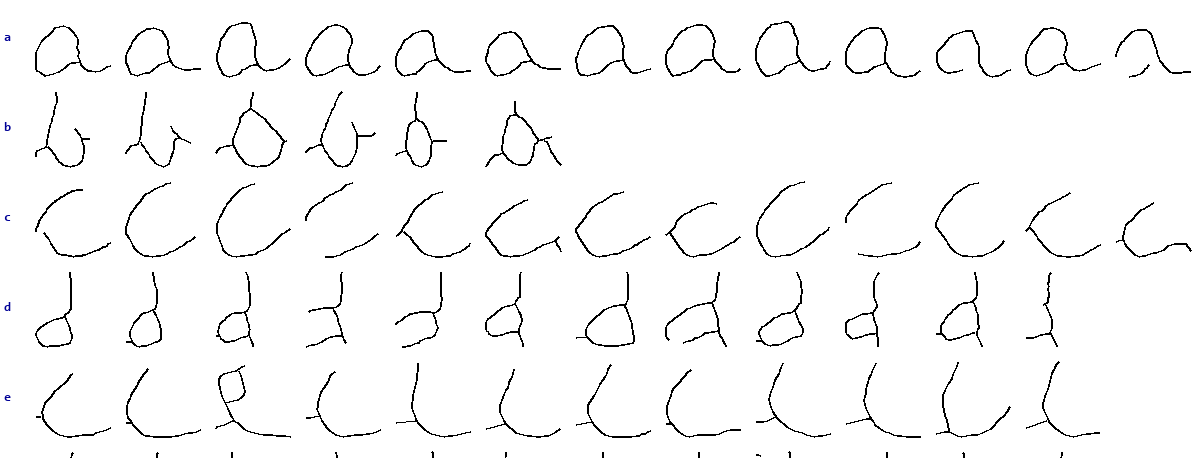
\includegraphics[width=0.78\linewidth]{Figures/w3_glyphs153_ae.png}
\caption{Stored variants of the letters a, b, c, d and e of writer 153, a strongly joined hand; each row is one character with up to 12 variants, the short tails at the sides being remains of ligatures.}
\label{fig:sty-glyphs}
\end{figure}

\subsubsection{Style statistics and permanent storage}
\label{sec:sty-stats}

Besides glyphs, the profile holds measured numbers: slant, pixel x-height, ascender and descender reach, word gap, and \emph{connectedness}, the fraction of adjacent letter pairs whose connection flag was set during tracing. Table~\ref{tab:sty-writers} shows the diversity this is built to reproduce --- slant $-10.5^\circ$ to $42.0^\circ$, connectedness 0.195 to 0.968, word gap 0.94 to 2.68 x-heights across the thirteen writers --- which is requirement R1's diversity target, and the thirteen files (about 4.8\,MB total) load when the server starts.

\begin{table}[!htbp]
\centering
\fontsize{7.5}{9}\selectfont
\setlength{\tabcolsep}{2.5pt}
\begin{tabular}{|l|r|r|r|r|r|r|r|}
\hline
\textbf{Writer} & \textbf{Lines} & \textbf{Slant ($^\circ$)} & \textbf{$x_h$ (px)} & \textbf{$A$} & \textbf{$D$} & \textbf{Gap} & \textbf{Conn.} \\
\hline
150 & 61 & $-4.5$ & 47 & 1.58 & $-0.72$ & 1.33 & 0.343 \\
151 & 58 & 33.0 & 22 & 2.69 & $-1.09$ & 1.59 & 0.968 \\
153 & 66 & 30.0 & 33 & 1.59 & $-1.10$ & 1.59 & 0.961 \\
384 & 54 & 4.5 & 43 & 1.93 & $-0.71$ & 1.37 & 0.500 \\
552 & 47 & $-10.5$ & 32 & 1.62 & $-0.56$ & 1.53 & 0.609 \\
dylan & 79 & $-6.0$ & 26 & 1.68 & $-0.62$ & 1.79 & 0.195 \\
thiya & 48 & 30.75 & 15 & 2.24 & $-1.00$ & 1.65 & 0.962 \\
yeukita & 74 & 0.0 & 27 & 1.45 & $-0.58$ & 0.94 & 0.417 \\
\hline
\end{tabular}
\caption{Representative rows of the thirteen stored style profiles (full table, Appendix~\ref{sec:app-syn}): kept lines, slant, pixel x-height, ascender $A$, descender $D$, word gap in x-heights, and connectedness.}
\label{tab:sty-writers}
\end{table}

\begin{figure}[htb]
\centering
\fbox{\parbox[c][4cm]{0.75\linewidth}{\centering [PLACEHOLDER --- scatter or bar plot of connectedness vs.\ reproduced character accuracy across the thirteen writers]}}
\captionsetup{singlelinecheck=false,justification=justified}
\caption{Placeholder: connectedness (Table~\ref{tab:sty-writers}) plotted against each writer's reproduced character accuracy from Table~\ref{tab:syn-evid}, to show quantitatively that the most joined hands are the hardest to reproduce.}
\label{fig:sty-conn-fig}
\end{figure}

\mustdo{\emph{The builder's \texttt{ExtractLineGlyphs} currently raises an import error} (a stale reference to a function moved during the restructuring of \texttt{TrainText.py}), so no new writer can presently be added and none of the thirteen stored profiles can be regenerated from the page images; the stored profiles themselves are unaffected and still load correctly. \texttt{legibilityLambda} is also absent from all thirteen stored files, so the system synthesises every writer at $\lambda=0$ until the tuner is re-run (Section~\ref{sec:syn-limits}).}

\subsubsection{Synthesis: choosing and placing a glyph}
\label{sec:syn-glyph}
\label{sec:syn-place}

The synthesiser takes text, a style profile, a pen size $x_{\mathrm{mm}}$ in millimetres and a random seed, and returns a \emph{trajectory}, pen-down polylines in millimetres; geometry stays in x-height units until one multiplication at the end, so one profile serves any pen size. Requirement R1 pulls in two directions at once: handwriting that resembles the writer argues for always using the writer's own letters, while handwriting that can be read argues for replacing the writer's worst letters with something clearer. The parameter $\lambda\in[0,1]$ is the single control that sets where a writer sits between those two. The obvious way to trade them off, blending the writer's glyph and a clear \emph{anchor} glyph geometrically, is \emph{not} used, because an average of two different pen strokes is usually not a valid letter at all; instead $\lambda$ scales the \emph{probability} that a chosen variant is replaced by the anchor outright, so every letter drawn is always a real letterform.

Global shear, join probability and line pitch follow from the profile (Equation~\ref{eq:syn-global}); among a writer's own variants for one character the choice is weighted by rank and, when joining, by how well the variant's entry height matches where the pen already is; the anchor-substitution probability is Equation~\ref{eq:syn-swap}; and placement is Equation~\ref{eq:syn-place-eq}:
\begin{align}
\theta_{\mathrm{cap}}&=45^\circ-19^\circ\lambda,\quad\sigma=\tan\!\bigl(\operatorname{clip}(\theta_{\mathrm p},\pm\theta_{\mathrm{cap}})\bigr)+\Delta_\sigma,\quad p_{\mathrm j}=\min(c,1),\label{eq:syn-global}\\
P_{\mathrm{swap}}(\lambda,d)&=\begin{cases}1&d\ge0.55,\\0&\lambda\le10^{-3},\\0.06\,\lambda&d\le0.12,\\\operatorname{clip}\bigl(\lambda\,(0.55+0.9\,b),0,1\bigr),\ b=\operatorname{clip}\bigl(\tfrac{d-0.12}{0.43},0,1\bigr)&\text{otherwise,}\end{cases}\label{eq:syn-swap}\\
X&=P_x+(\ell+x+\sigma_g\,y)\,x_{\mathrm{mm}},\qquad Y=P_y+(y+\delta_g)\,x_{\mathrm{mm}}.\label{eq:syn-place-eq}
\end{align}
A variant beyond prior distance $d=0.55$ is replaced \emph{unconditionally}, whatever $\lambda$; one closer than $d=0.12$ is kept almost always; between those the probability rises with both $d$ and $\lambda$. Below $\lambda=10^{-3}$ substitution switches off entirely, so a writer tuned to zero keeps even their marginal letters. When a writer's medoid itself is too malformed to serve as the anchor, a hand-designed single-stroke skeleton (joined cursive or upright print, re-proportioned to that writer's ascender and descender reach) is used instead, reading back at about 96\,\% character and 84\,\% word accuracy, which is what makes it a usable floor.

Treating connectedness $c$ as a hard threshold, joining every pair above it, was tried first and fused whole words into unbroken blobs, losing the irregularity that makes a hand look human; it is used as a per-pair \emph{probability} $p_{\mathrm j}$ instead. Measured over a design-stage probe, the anchor share this produces ran from 0\,\% for writer 552 to 76\,\% for writer 151, the most joined hand of the set. One pseudo-random stream seeded by the seed argument supplies every draw, so the arguments fix the output completely; at the jitter amplitude the search uses, a letter is perturbed by about a $1.1^\circ$ rotation, a 2.5\,\% scale change and under 0.05\,mm translation. \emph{Style calibration}: because glyphs are placed one instance at a time, an assembled line does not automatically reproduce the writer's own line-level slant and ascender reach (writer 150's ascenders came out about 7\,\% too tall, writer 551's slant about $9^\circ$ too steep against real lines), so a fixed probe sentence is synthesised once per writer and three fixed-point iterations of Equation~\ref{eq:syn-cal} adjust the shear shift $\Delta_\sigma$ and the scale factors $K_A$, $K_D$ until the probe matches the stored real-line reference values:
\begin{equation}
\Delta_\sigma\leftarrow\Delta_\sigma+\tan\theta_{\mathrm{ref}}-\tan\theta_{\mathrm{got}},\quad K_A\leftarrow\operatorname{clip}\Bigl(K_A\frac{A_{\mathrm{ref}}-1}{A_{\mathrm{got}}-1},0.5,1.6\Bigr),\quad K_D\leftarrow\operatorname{clip}\Bigl(K_D\frac{D_{\mathrm{ref}}}{D_{\mathrm{got}}},0.5,1.6\Bigr),
\label{eq:syn-cal}
\end{equation}
with ``ref'' the stored real-line value and ``got'' the probe's measured value by the estimators of Section~\ref{sec:sty-trace}, each correction clipped to bound its effect.

\begin{figure}[htb]
\centering
\fbox{\parbox[c][4.5cm]{0.85\linewidth}{\centering [PLACEHOLDER --- the same letter drawn at $\lambda=0$, $\lambda=0.5$ and $\lambda=1$ for one strongly joined writer, each candidate's prior distance $d$ and swap probability printed beside it]}}
\captionsetup{singlelinecheck=false,justification=justified}
\caption{Placeholder: the legibility sweep of Equation~\ref{eq:syn-swap} on one writer's worst-scoring letter, from the writer's own glyph through partial anchor substitution to the full anchor, with $P_{\mathrm{swap}}$ plotted against prior distance $d$ for several $\lambda$ as an inset curve.}
\label{fig:syn-swap-fig}
\end{figure}

\subsubsection{Best-of-$N$ search with joint scoring}
\label{sec:syn-search}

Single draws vary in quality, so a line is drawn $N$ times and the best kept; the score must use both judges together, because selecting by text accuracy alone raised legibility but lowered writer identification for some writers in a design-stage probe, since the most legible of several random draws need not be the most characteristic.

For a rendered candidate $I$, with $\hat y(I)$ the recogniser's greedy reading and $y$ the intended text, the text term $a(I)$ below is built from the Levenshtein edit distance~\cite{levenshtein1966}, the smallest number of insertions, deletions and substitutions turning one string into the other,
\begin{equation}
a(I)=\max\Bigl(0,1-\frac{\mathrm{Lev}(\hat y(I),y)}{|y|}\Bigr),\quad w(I)=\mathrm{softmax}\bigl(f_{\mathrm{wid}}(I)\bigr)_{a^\star},\quad S(I)=\frac{2\,a(I)\,w(I)}{a(I)+w(I)},
\label{eq:syn-score}
\end{equation}
the harmonic mean of recogniser accuracy and shape-classifier confidence in the target writer $a^\star$, dominated by whichever is smaller, so a candidate cannot win on one criterion while failing the other.

The search has two loops (Figure~\ref{fig:syn-search}): the first draws up to $N$ candidates and keeps the best by $S$; the second, a \emph{repair} loop of at most three rounds, forced-aligns the intended text to the best image, pins the two worst-scoring characters to the anchor, re-synthesises the whole line, and accepts the result only if $S$ strictly improves, so a repair that fixes a letter but makes the line resemble another writer is rejected. $N$ is 6 as the function default, 14 for design-stage measurements, 20 as the web default and 30 in the evaluation script; the cost is entirely judge-bound, synthesising a candidate costing 11 to 16\,ms against 0.5 to 4\,s to score it, so $N$ rather than the construction itself sets the reproduction time of requirement R3.

\begin{figure}[!htbp]
\centering
\begin{tikzpicture}[node distance=3.2mm and 6mm]
\node[w3io] (in) {text, profile, writer $a^\star$, seed base, $N$};
\node[w3box,below=of in] (syn) {synthesise candidate $k$, score by Equation~\ref{eq:syn-score}};
\node[w3dec,below=4.5mm of syn] (loop) {best reaches 0.99,\\or $k=N-1$?};
\node[w3box,below=of loop] (align) {repair: align, pin two weakest\\characters to anchor, re-synthesise};
\node[w3io,below=of align] (out) {best trajectory (at most 3 repair rounds)};
\draw[w3arr] (in) -- (syn);
\draw[w3arr] (syn) -- (loop);
\draw[w3arr] (loop.west) -- node[w3lab,above,pos=0.3]{no} ++(-14mm,0) |- (syn.west);
\draw[w3arr] (loop) -- node[w3lab,right]{yes} (align);
\draw[w3arr] (align) -- (out);
\end{tikzpicture}
\caption{Control flow of the candidate search of \texttt{SynthesizeJointBestOf}, simplified from the full state machine; both the main loop and the repair loop use the joint score of Equation~\ref{eq:syn-score}.}
\label{fig:syn-search}
\end{figure}

Table~\ref{tab:syn-evid} lists the measurements that motivated the design, over six novel sentences, two seeds and ten writers. Joint best-of-$N$ at $N=14$ reached 97.5 / 95.8\,\% writer identification and 81.6 / 81.4\,\% character accuracy (direct / through G-code); on a matching comparison of identical words, synthesis costs 7.4 percentage points of character accuracy against the writers' own real handwriting (89.0\,\% vs.\ 81.6\,\%) and more than 1.5 times the word accuracy (70.5\,\% vs.\ 46.7\,\%), which locates the loss in spacing and word boundaries rather than in letterforms.

\begin{table}[!htbp]
\centering
\fontsize{8}{9.6}\selectfont
\setlength{\tabcolsep}{4pt}
\begin{tabularx}{\linewidth}{|X|c|c|}
\hline
\textbf{Stage} & \textbf{Writer ID, direct / G-code (\%)} & \textbf{Char.\ acc., direct / G-code (\%)} \\
\hline
Plain synthesis after label and glyph fixes & 79.2 / 80.0 & 75.9 / 76.3 \\
Text-only best-of-$N$ with plain repair & 76.7 / 73.3 & 83.8 / 82.7 \\
Joint best-of-$N$, $N=14$ & 97.5 / 95.8 & 81.6 / 81.4 \\
\hline
Final system, 13 writers, 3 sentences, $N=8$ & 92.3 / 89.7 & 79.2 / 79.2 \\
\hline
Matching comparison: writers' own real handwriting & not applicable & 89.0 / --- \\
Matching comparison: synthesis of the same words & not applicable & 81.6 / --- \\
\hline
\end{tabularx}
\caption{Measurements that motivated the design (upper block) and the final system (lower blocks). Only the two matching-comparison rows are independent of the search and so the figures to trust most directly; the rest are qualified by Section~\ref{sec:syn-limits}.}
\label{tab:syn-evid}
\end{table}

\begin{figure}[!htbp]
\centering

\includegraphics[width=0.95\linewidth]{Figures/w3_synth_150.png}\\[1pt]

\includegraphics[width=0.95\linewidth]{Figures/w3_synth_153.png}
\caption{Synthesised line for writer 150 (upper, printed hand, read back with three small errors) and writer 153 (lower, joined hand, read back with several letter errors), one seed and candidate each, rendered from an end-to-end run.}
\label{fig:syn-lines}
\end{figure}

\subsubsection{Alternatives considered}

A recurrent sequence generator with attention and a mixture-density stroke output, the approach that first generated convincing on-line handwriting from a recurrent network~\cite{graves2013}, needs hundreds to thousands of lines of on-line pen data per writer, where only 47 to 130 scanned lines exist per writer here; a from-scratch version trained on skeleton-derived strokes learned slant, roundness and connectedness but no legible letters, and was rejected. Adversarial and diffusion generators conditioned on a style exemplar~\cite{kang2020,dai2024} need less data through pre-training but emit a raster needing the same thinning to vectorise, cannot control size, slant and spacing as explicit numbers, and took 35 to 45\,s per line in a trial against 3 to 8\,s for glyph synthesis, so they were parked. The approach closest in spirit to the one built here is exemplar-based synthesis from a writer's own captured letterforms~\cite{haines2016}, re-assembling stored shapes rather than generating pixels from a learned distribution; the glyph library needs about nine pages per writer and no training, exposes every parameter as an explicit number, and costs about 15\,ms per candidate, which suits a single-board computer with no accelerator; its one clear weakness is joined hands, whose joins are necessarily lost by the character-cutting of Section~\ref{sec:sty-forced}.

\subsubsection{Known faults and limitations}
\label{sec:syn-limits}

\begin{enumerate}\setlength{\itemsep}{0pt}\setlength{\parskip}{0pt}
\item \emph{The legibility mechanism is inert as submitted}, because \texttt{legibilityLambda} is absent from all thirteen stored profiles and defaults to zero, so $\lambda=0$ on the live path: only the unconditional substitutions at $d\ge0.55$ fire, and every $\lambda$-dependent figure above describes a tuned configuration that is not what the delivered profiles currently run.
\item Every figure after the search is introduced is the opinion of the very networks that selected the output: the search loads the same weight files as the measurement, so the values show the pipeline can satisfy its two judges, not that an independent reader would agree.
\item $\lambda$, the anchor threshold and $N$ were tuned on the same sentences Section~\ref{sec:results} measures, and the style calibration of Section~\ref{sec:syn-glyph} measures both sides with the same estimator, so its agreement is partly self-fulfilling.
\item Writers 151 and 552, the two most joined hands, reach only 53 and 56\,\% character accuracy through G-code against about 84\,\% for the other eleven, the clearest limitation of the exemplar approach and a direct consequence of the cutting problem of Section~\ref{sec:sty-forced}.
\item Cutting a joined line destroys how a letter changes shape with its neighbours, which is the underlying reason writers 151 and 551 are reproduced least legibly.
\end{enumerate}


\subsection{Design reconsiderations}
\label{sec:later}

The four sections above describe each subsystem as delivered, but four of those designs are not what was built first: each replaced an earlier version once the complete chain existed and the output could be measured end to end, which is the point at which faults invisible inside a single subsystem became apparent. They are collected here, separately from the component descriptions above, because each is a change of \emph{approach} rather than a correction of code, and because the reason for each lies outside the subsystem it altered. Several of these reconsiderations are referenced from Sections~\ref{sec:writerid} and~\ref{sec:synthesis} above and are given their full justification here.

\subsubsection{A second writer classifier, judging shape instead of ink}
\label{sec:later-strokenorm}

The first writer classifier was trained on grey-scale crops and read real held-out lines at 99.78\,\% over 1358 lines, which satisfied requirement R2 on photographed pages. Measured on \emph{synthesised} output, however, the same classifier identified the intended writer in only about 28\,\% of trials. The cause is a property of the machine rather than of the network: the gantry draws every stroke with one pen at one width and one pressure, whereas real handwriting carries a thickness and an ink density that a convolutional network exploits readily when the training lines are few. A classifier that leans on those cues therefore predicts neither what the machine can draw nor how a reader recognises a hand, which is by geometry.

The response was to train a second classifier of the same architecture on stroke-normalised crops, in which the ink is thinned to a centre line and redrawn at a constant width proportional to the letter height, so thickness is removed by construction (Section~\ref{sec:wid-strokenorm}). This is the reconsideration that matters most for requirement R1: style can be judged, and reproduced, on geometry alone once pen pressure and width are taken out of the comparison. The two classifiers are used for different purposes, and the division is kept throughout the system: the ink classifier serves real photographed pages, and the shape classifier serves the candidate search of Section~\ref{sec:syn-search}. Neither replaced the other, so the writer-identification block carries two sets of weights rather than one, at the cost of double the training and storage for a capability the first classifier could not provide at all.

\subsubsection{End-to-end training in place of a frozen backbone}
\label{sec:later-endtoend}

The shape classifier was first trained by fitting only the 13\,645 parameters of its head on feature vectors extracted once from a frozen backbone. That recipe is a training fault, set out in Section~\ref{sec:writerid}: because the features were extracted once, no augmentation was re-sampled between epochs and every line contributed the same four fixed vectors for all 500 epochs. Training all 966\,445 parameters end to end instead raised the same measurement from 83.36\,\% to 93.67\,\% on the same 1358 real lines, and removed a failure in which 118 of one writer's 148 lines had been assigned to a single neighbour. Every figure quoted for the shape classifier elsewhere in this report is from the end-to-end model; the frozen-head figures describe the superseded one, and are kept here only as the evidence for why the change was made.

\subsubsection{Selecting a candidate on both criteria instead of legibility alone}
\label{sec:later-joint}

The candidate search first kept whichever of the $N$ draws the text recogniser read most accurately. That raised legibility and, for some writers, lowered writer identification, because the most legible of several random draws has no reason also to be the most characteristic. The score was therefore changed to the harmonic mean of the recogniser's character accuracy and the shape classifier's confidence in the intended writer, Equation~\ref{eq:syn-score}, dominated by whichever of the two is smaller, so a candidate cannot win on one criterion while failing the other. The repair loop was changed for the same reason, accepting a repaired line only when the joint score improves, so a repair that fixes a letter but makes the line resemble another writer is rejected rather than taken. The evidence for both changes is Table~\ref{tab:syn-evid}.

\subsubsection{Line-level style calibration}
\label{sec:later-cal}

Glyphs are stored and placed one instance at a time, so a line assembled from them does not automatically reproduce the writer's line-level slant and ascender reach. The calibration of Section~\ref{sec:syn-glyph} was added to correct that drift, measuring a rendered probe with the same functions that measured the writer's real pages and returning a shear and reach correction. The drift it corrects was itself measured before the change: writer 150's ascenders came out about 7\,\% too tall and writer 551's slant about $9^\circ$ too steep against their own real lines. Unlike the other three changes, this one has no clean before-and-after pair in Table~\ref{tab:syn-evid}, so its benefit rests on the probe agreeing with the stored reference rather than on a judge's score, and Section~\ref{sec:syn-limits} records that this agreement is partly self-fulfilling, since it is measured by the same estimator on both sides.
\mustdo{measure writer identification and character accuracy with the calibration of Section~\ref{sec:syn-glyph} disabled and enabled, over the same sentences and seeds as the other rows of Table~\ref{tab:syn-evid}, so that this change carries the same kind of evidence as the other three.}

\subsubsection{A reconsideration not yet carried out: detecting the need for an anchor automatically}

One further change was identified during the glyph-library investigation of this project but has not been implemented in the delivered system, and is recorded here as a design reconsideration still open rather than as a completed change, since the distinction between what was changed and what is merely proposed matters to how this section should be read. The anchor-substitution mechanism of Section~\ref{sec:syn-glyph} is driven entirely by the per-glyph prior distance of Equation~\ref{eq:sty-prior} and the single tuned parameter $\lambda$, applied uniformly within a writer. An examination of the glyph cutting and the cross-writer prior distribution for the most strongly joined personal writer in this project's data showed that her low connectedness-adjusted legibility is not a scattered collection of individually poor letters but a structural property of her hand: her forced-alignment cuts fall through genuine strokes far more often than for a lightly joined writer, because her connectedness statistic of 0.962 (Table~\ref{tab:sty-writers}) leaves almost no low, thin ligature for Equation~\ref{eq:sty-cut} to find. The reconsideration this suggests is to use the writer's \emph{own} connectedness and the \emph{distribution} of her glyphs' prior distances, rather than $\lambda$ alone, to decide automatically whether a writer needs anchor substitution forced on by default, instead of relying on a value tuned by hand per writer. A substitution experiment on this writer's own held-out sentences, forcing full anchor use rather than the tuned $\lambda$, raised the shape classifier's confidence in her identity from 63--77\,\% to 94\,\% and gave a modest further gain in character accuracy, which is evidence the direction is worth pursuing, though word accuracy stayed poor regardless of the glyph source, pointing to a second, separate limitation in the synthesiser's joining geometry that this reconsideration alone would not fix.
\mustdo{implement and measure the connectedness-triggered default described here across all thirteen writers, not only the one case it was explored on.}

\mustdo{confirm that these five are the complete set of reconsiderations made or identified during the project, and add any others that belong here --- for example a change to the segmentation thresholds, to the number of writers, or to the requirement allocation --- each with what was measured before and after.}


\subsection{Software design and system integration}
\label{sec:system}

% Compact display spacing for this subsection only; restored at the end of the file.
\begingroup
\setlength{\abovedisplayskip}{4pt}\setlength{\belowdisplayskip}{4pt}
\setlength{\abovedisplayshortskip}{2pt}\setlength{\belowdisplayshortskip}{2pt}

This subsection describes how the blocks of Sections~\ref{sec:gantry} to~\ref{sec:later} form one application on the single-board computer, which runs a web server exposing them to a browser. All are Python programs written for this project; only the camera interface, the pin interface and the transport of web requests come from libraries, with the one exception below.

\subsubsection{Process flow and start-up}

Figure~\ref{fig:sys-flow} is the process flow of the two run-time modes. At start-up the application loads the thirteen profiles and the three networks, each a from-scratch array-arithmetic evaluation of trained weights (Sections~\ref{sec:textrec} and~\ref{sec:writerid}); the reproduction chain then calls the synthesiser once with both judges passed in and refuses to send unless calibration has succeeded in this session. Training is a third mode, the writers being pre-built files from offline programs. \mustdo{the board's address and connection to the laptop, the operating system and Python version, how the server is started, and the memory the loaded models use.}

\begin{figure}[!htbp]
\centering
\begin{tikzpicture}[x=1cm,y=1cm]
\tikzset{p/.style={w3box,text width=2.2cm,minimum height=1.0cm,font=\scriptsize},
         s/.style={w3store,text width=2.2cm,minimum height=0.85cm,font=\scriptsize},
         i/.style={w3io,text width=2.2cm,minimum height=0.85cm,font=\scriptsize}}
\node[p] (a1) at (0,0) {Read page: capture or upload};
\node[p] (a2) at (3,0) {Condition, segment lines};
\node[p] (a3) at (6,0) {Recogniser and ink classifier};
\node[p] (a4) at (9,0) {Mean writer probabilities};
\node[p] (a5) at (12,0) {Text, writer, confidence};
\node[p] (b1) at (0,-1.9) {Write page: text, writer, $N$};
\node[p] (b2) at (3,-1.9) {Best-of-$N$ synthesis};
\node[p] (b3) at (6,-1.9) {G-code and preview};
\node[p] (b4) at (9,-1.9) {Read-back by recogniser};
\node[p] (b5) at (12,-1.9) {Send to calibrated gantry};
\node[s] (prof) at (3,-3.25) {Thirteen style profiles (JSON)};
\node[i] (gan) at (12,-3.25) {Gantry, pen, switches};
\begin{scope}[on background layer]
\node[w3group,fit=(a1)(a5)(b1)(b5),inner sep=7pt] (srv) {};
\end{scope}
\node[font=\scriptsize\bfseries,anchor=south west] at (srv.north west) {One application on the ODROID N2+};
\foreach \u/\v in {a1/a2,a2/a3,a3/a4,a4/a5,b1/b2,b2/b3,b3/b4,b4/b5} \draw[w3arr] (\u) -- (\v);
\draw[w3arr] (prof) -- (b2);
\draw[w3arr] (b5) -- (gan);
\end{tikzpicture}
\caption{Process flow of the two run-time modes: classification above, reproduction below, the writer the upper chain identifies being what the lower chain is given. The profile builder of Section~\ref{sec:styleprofile} is offline and appears in neither.}
\label{fig:sys-flow}
\end{figure}

\paragraph{The inference path is library-free; the sample-crop warm-up is not.}
A recorded cold-boot import closure confirms that \texttt{torch}, \texttt{scipy}, \texttt{cv2} and \texttt{tensorflow} are reached by none of the three networks and none of the classification, synthesis, G-code and motion paths: every weight comes from a plain array archive and every layer is evaluated by the project's own array arithmetic. One path breaks that. The start-up warm-up, given as pseudocode in Figure~\ref{fig:sys-code-warm}, calls \texttt{WRH.SampleCrops} for every writer, and on a cache miss that helper imports \texttt{BuildStyleProfile}, \texttt{TrainAuthor} and \texttt{TrainText}; \texttt{WebRenderHelpers.py} prepends \texttt{Software/CNN} and its \texttt{AuthorReproductionStuff} to \texttt{sys.path}, so those names resolve to the \emph{retired} tree, whose \texttt{TrainText.py} and \texttt{TrainAuthor.py} import \texttt{torch}, \texttt{torchvision}, \texttt{pytesseract} and \texttt{scipy} at module level. \texttt{WebCache} as delivered has no glyph grid or crops for owen and thiya and none for abhinav, so the miss, and the import, happen on \emph{every} start. \mustdo{port the two sample-crop helpers into \texttt{CleanPipeline}, or pre-populate \texttt{WebCache} for owen, thiya and abhinav, so that no import reaches \texttt{Software/CNN}; then repeat the cold-boot closure on the board.}


\paragraph{Known inconsistency: the stored accuracy figures.}
One route computes nothing: it returns figures hard-coded in \texttt{Server.py}, several no longer agreeing with Section~\ref{sec:results} --- the ink-based classifier at 100.0\,\%, the stroke-normalised one at 96.7\,\% on real ink and 99.2\,\% on synthesised output, the recogniser at 89.4\,\% on real ink, and the pipeline at 99.2\,\% writer identification with 85.8\,\% and 84.1\,\% character accuracy direct and through G-code. The code is stale here, not the report, and the page displaying those figures contradicts the Results chapter. \mustdo{update the hard-coded accuracy block of \texttt{/api/model\_info} to the final figures of Section~\ref{sec:results}, or have the route read them from the evaluation output.}

\subsubsection{Timing chains of the two modes}

Requirement R4 limits the classification of $x$ characters by Equation~\ref{eq:sys-cls},
\begin{equation}
T_{\mathrm{cls}}=T_{\mathrm{cap}}+T_{\mathrm{seg}}+\sum_{\mathrm{lines}}\bigl(T_{\mathrm{text}}+T_{\mathrm{wid}}\bigr)\le2\ \mathrm{s}+0.025\,x\ \mathrm{s},
\label{eq:sys-cls}
\end{equation}
leaving both network passes 25\,ms per character, and R3 limits reproduction by Equation~\ref{eq:sys-rep},
\begin{equation}
T_{\mathrm{rep}}=T_{\mathrm{synth}}+T_{\mathrm{gcode}}+T_{\mathrm{motion}}\le4\,x\ \mathrm{s},\qquad T_{\mathrm{synth}}\approx N\,C,
\label{eq:sys-rep}
\end{equation}
with $C$ the cost of one candidate (Equation~\ref{eq:syn-cost}), $T_{\mathrm{gcode}}$ in milliseconds and $T_{\mathrm{motion}}$ the job time of Section~\ref{sec:gan-timing}; the calibration is excluded and $T_{\mathrm{synth}}$ included, the stricter reading of the proposal.
A budget is only a design once it is apportioned, and Table~\ref{tab:app-budget} in Appendix~\ref{sec:app-sys} gives the allowance this design assigned to each stage of Equations~\ref{eq:sys-cls} and~\ref{eq:sys-rep} against the figure later measured for it.
The apportionment follows from the structure of the chain rather than from the measurements: the two network terms were given the whole per-character allowance of R4, being the only terms that grow with $x$, which leaves the fixed two seconds for capture, conditioning and segmentation; and in R3 the physical writing was given three quarters of the per-character allowance, being the one term that no faster computer can reduce.
Read against that apportionment, four of the five stages are inside their allowance and the whole R4 shortfall sits in page segmentation, at twelve to thirty-five times what it was allowed.
Table~\ref{tab:sys-timing} lists the stages, and \emph{no stage was timed on the single-board computer}: a 56-character sentence allows 224\,s, while the search alone took 23 to 137\,s at $N=14$ on the laptop and the motion model gives 2.4 to 2.8\,s per character, so R3 and R4 are not claimed to be met. \mustdo{the timings of the stages on the single-board computer, listed in Table~\ref{tab:sys-timing}.}

\begin{table}[!htbp]
\centering
\fontsize{8}{9.3}\selectfont
\setlength{\tabcolsep}{3.5pt}\renewcommand{\arraystretch}{1.02}
\begin{tabularx}{\linewidth}{|p{3.2cm}|X|}
\hline
\textbf{Stage} & \textbf{Known information and value to be supplied} \\
\hline
Capture, conditioning and segmentation & Framing by the user, five discarded frames without preview; whole page on the board. \mustdo{time from pressing capture to the stored image.} \mustdo{conditioning and segmentation time per page on the board.} \\
\hline
Recognition and writer classification & Two passes of about $4\times10^9$ multiply--accumulate operations per line. \mustdo{time per line on the board and the total for the R4 test paragraph.} \\
\hline
Synthesis, G-code and preview & Synthesis time is returned in the server response (laptop values in Table~\ref{tab:syn-cost}); the generator and preview are milliseconds, not measured. \mustdo{synthesis time on the board for the $N$ used in the demonstration.} \\
\hline
Gantry motion & Model 2.4 to 2.8\,s per character (Section~\ref{sec:gan-timing}). \mustdo{stopwatch time of a sentence of known length, from send to the final pen lift.} \\
\hline
\end{tabularx}
\caption{Stages of the timing chains of the two modes and the measurements still missing.}
\label{tab:sys-timing}
\end{table}

Complete code has been submitted separately on the AMS.
\mustdo{confirm which archive and revision was submitted on the AMS.}

\endgroup

